\lstdefinestyle{MethodenListe}{
    language   = Python,
    numbers    = none,
    belowskip  = 0.25em,
    basicstyle = \tt\small
}

\lstdefinestyle{MethodenListeKlein}{
    language   = Python,
    numbers    = none,
    belowskip  = 0.25em,
    basicstyle = \tt\footnotesize
}

%%% Folie
\begin{frame}{Lernziele}
    \begin{block}{Hardware}
        \begin{itemize}
            \footnotesize
            \setlength\itemsep{.5em}

            \item Die am Raspberry Pi nutzbaren Signalarten erklären können
            \item Die Hardwareschnittstellen des Raspberry Pi nutzen können
            \item Analoge und digitale Sensoren und Aktoren verbinden können
            \item Stromstärken und Spannungen an den Raspberry Pi anpassen
            \item Funktionsweise der seriellen Kommunikation erklären können
            \item Externe Bausteine und Microcontroller seriell anbinden können
        \end{itemize}
    \end{block}

    \begin{block}{Programmierung}
        \begin{itemize}
            \footnotesize
            \setlength\itemsep{.5em}

            \item Bibliotheken für die hardwarenahe Programmierung in Python kennen
            \item Die GPIO-Schnittstelle des Raspberry Pi programmieren können
            \item Verschiedene Programmierstile abgrenzen und bewerten können
        \end{itemize}
    \end{block}
\end{frame}

%-------------------------------------------------------------------------------
\section{Hardwareschnittstellen des Raspberry Pi}
%-------------------------------------------------------------------------------


%%% Folie
{
\scriptsize

\begin{frame}{Anschlüsse am Raspberry Pi}
        \Justified{
            Aufgrund seiner hohen Rechenleistung (vergleichbar mit einem mittleren Smartphone
            oder älterem Desktopcomputer) und seiner Vielzahl elektrischer Schnittstellen
            eignet sich der Rasbperry Pi für vielfältige eingebettete Anwendungen. Mit einer
            kleinen Einschränkung (Analogsignale nur mit Hilfsschaltungen möglich und auch
            der Audioausgang nutzt ein gefiltertes PWM-Signal statt einem echten D/A-Wandler),
            können fast alle typischen Bauteile mit dem Raspberry Pi verbunden werden.
        }

        %~ \smallskip

        \begin{center}
            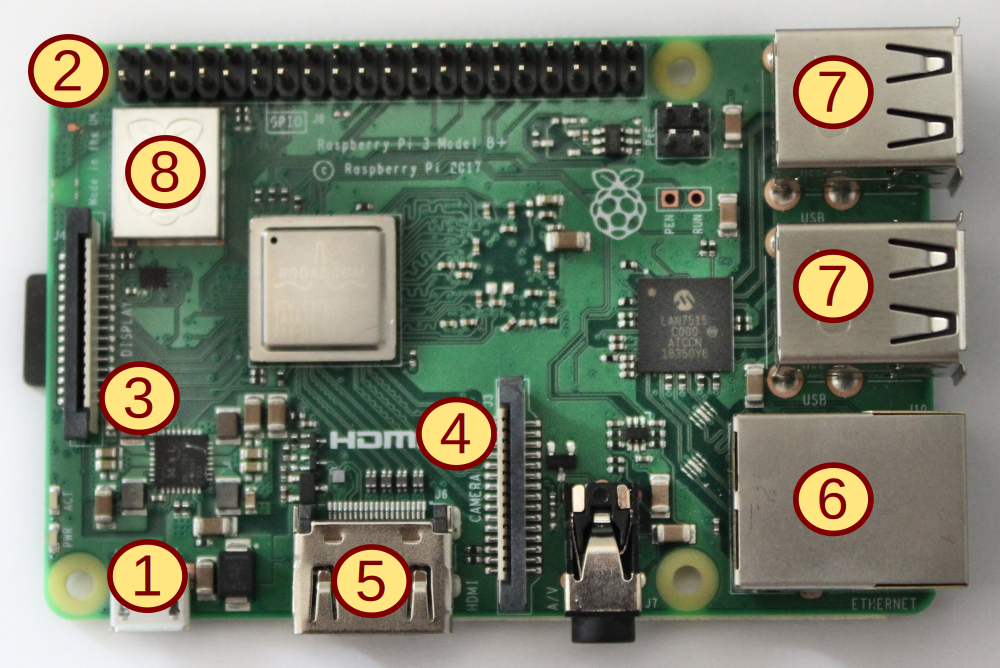
\includegraphics[height=0.5\textheight]{img/raspberry_anschluesse}
        \end{center}

        %~ \smallskip

        \begin{columns}
            \begin{column}[T]{.5\textwidth}
                \begin{enumerate}
                    \item Mini-USB Stromversorgung
                    \item J8 GPIO-Header
                    \item Display Serial Interface
                    \item Camera Serial Interface
                \end{enumerate}
            \end{column}
            \begin{column}[T]{.5\textwidth}
                \begin{enumerate}
                    \setcounter{enumi}{4}   % Zielwert - 1
                    \item HDMI-Bildschirmanschluss
                    \item LAN-Netzwerkanschluss
                    \item USB (4 Stück)
                    \item WiFi, Bluetooth
                \end{enumerate}
            \end{column}
        \end{columns}
\end{frame}
}

%%% Folie
{
\footnotesize

\begin{frame}{Der J8 GPIO-Header im Detail}
        \begin{columns}
            \column[b]{.5\textwidth}
            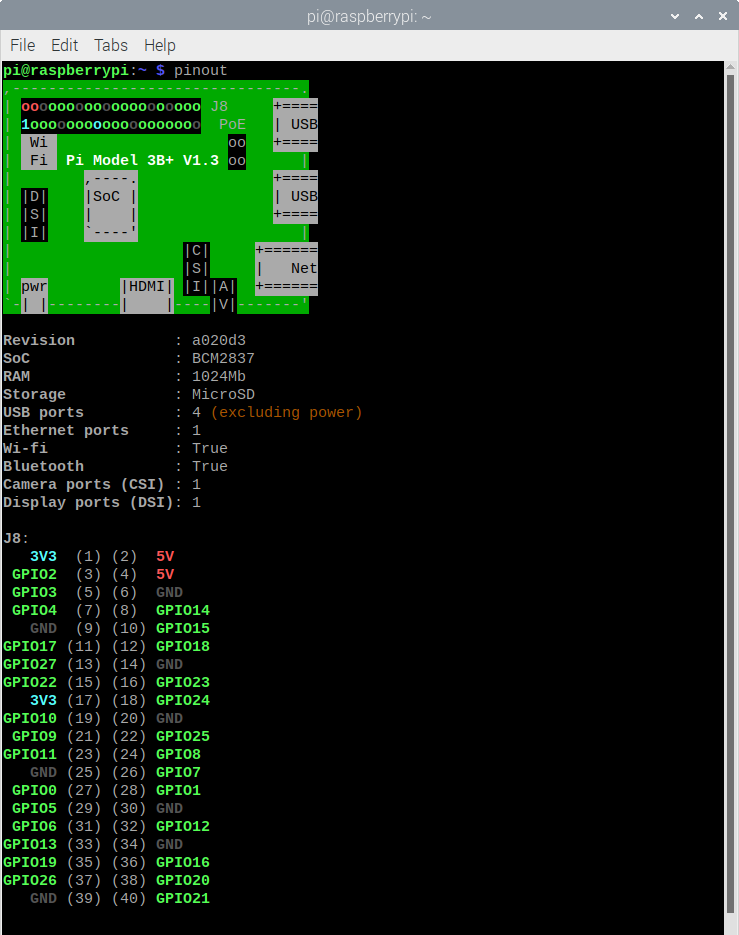
\includegraphics[height=.7\textheight]{img/pinout}
            %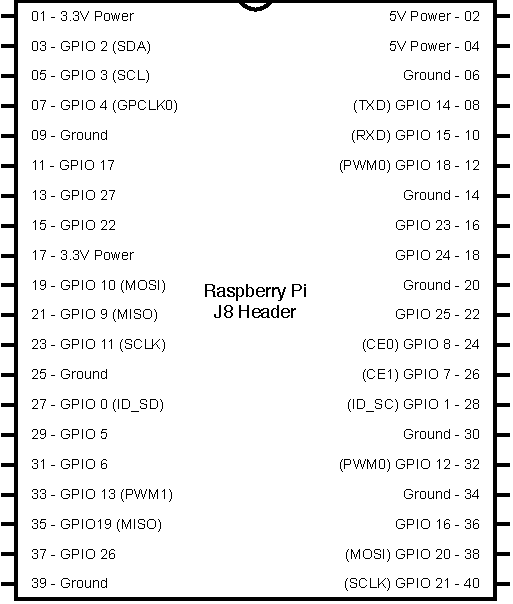
\includegraphics[width=\textwidth]{img/raspberry_j8}

            \medskip
            \LinkButton{https://pinout.xyz/}{Raspberry Pi Pinout Guide}

            \column[b]{.5\textwidth}
            \begin{block}{Stromquellen}
                \begin{itemize}
                    \item 5V Power
                    \item 3.3V Power
                    \item Ground (Masse)
                \end{itemize}
            \end{block}

            \begin{block}{Digitale Ein-/Ausgänge}
                \begin{itemize}
                    \item GPIO
                    \item Pulsweitenmodulation
                    \item Asynchron serielle Kommunikation
                    \item Synchron serielle Kommunikation \\ (SPI, I²C, I²S, 1-Wire)
                \end{itemize}
            \end{block}

            \begin{alertblock}{Keine analogen Ein-/Ausgänge!}
            \end{alertblock}
        \end{columns}
\end{frame}
}

%%% Folie
\begin{frame}{Häufig vorkommende Signalarten}
        \begin{columns}
        \column[b]{.5\textwidth}
        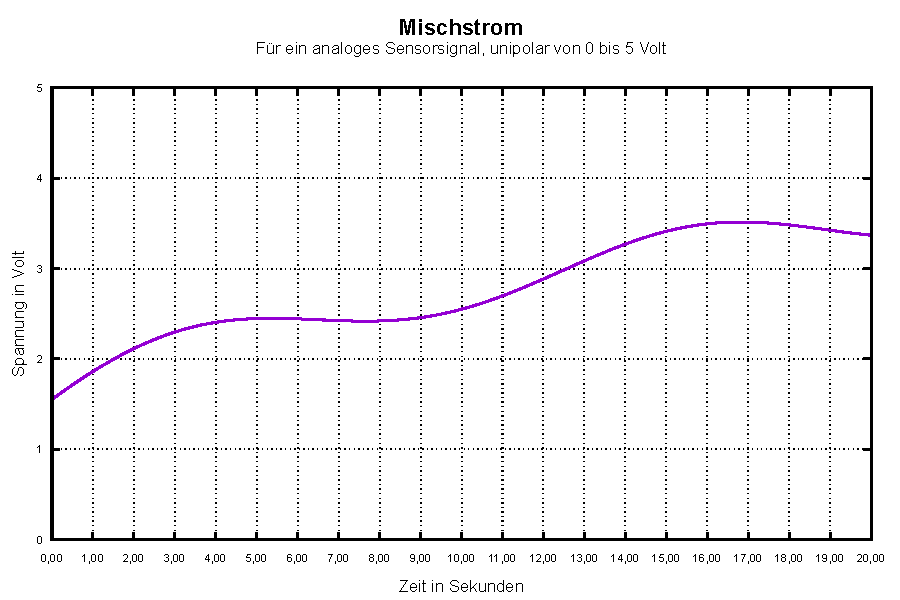
\includegraphics[width=\textwidth]{img/strom-analogsensor} \\

        \column[b]{.5\textwidth}
        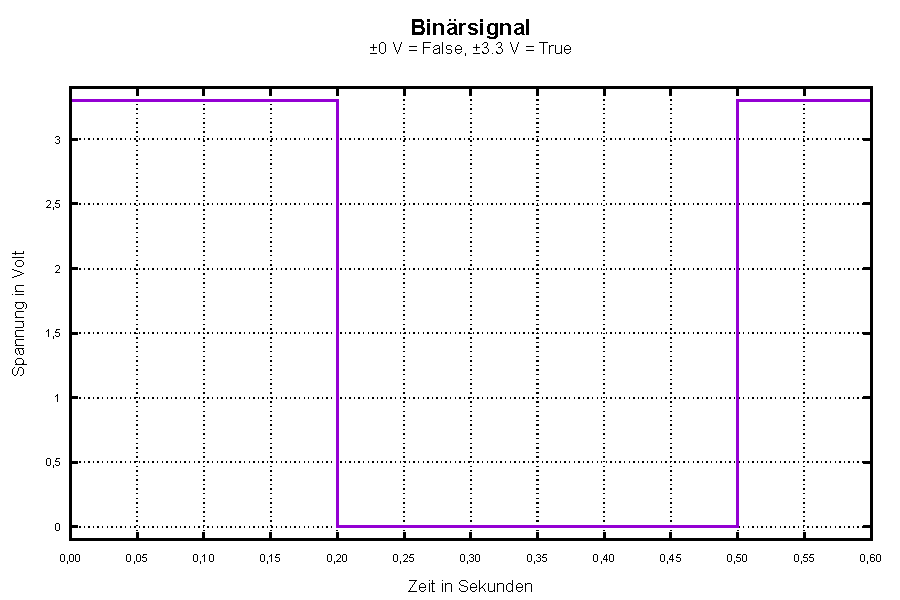
\includegraphics[width=\textwidth]{img/strom-binary} \\
    \end{columns}

    \bigskip

    \begin{columns}
        \column[b]{.5\textwidth}
        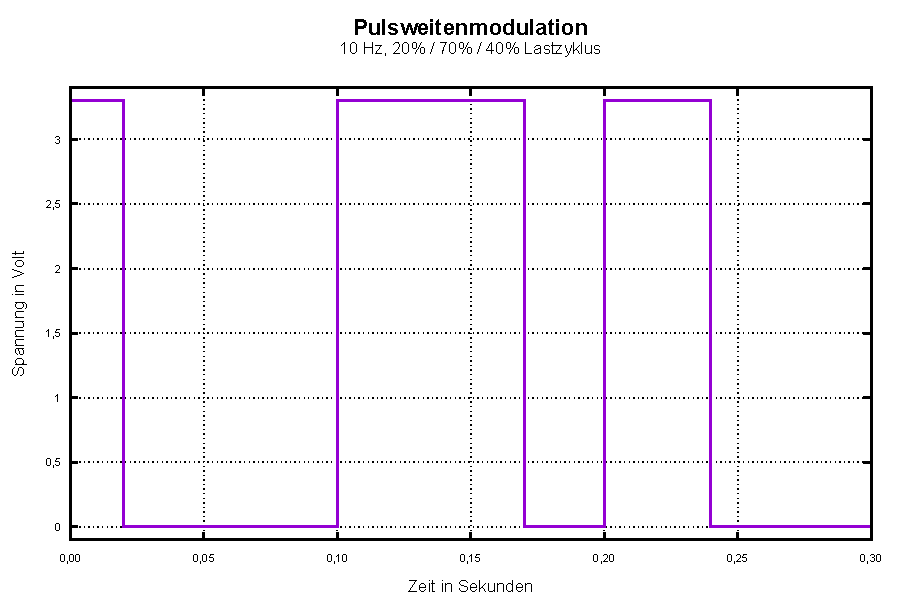
\includegraphics[width=\textwidth]{img/strom-pwm} \\

        \column[b]{.5\textwidth}
        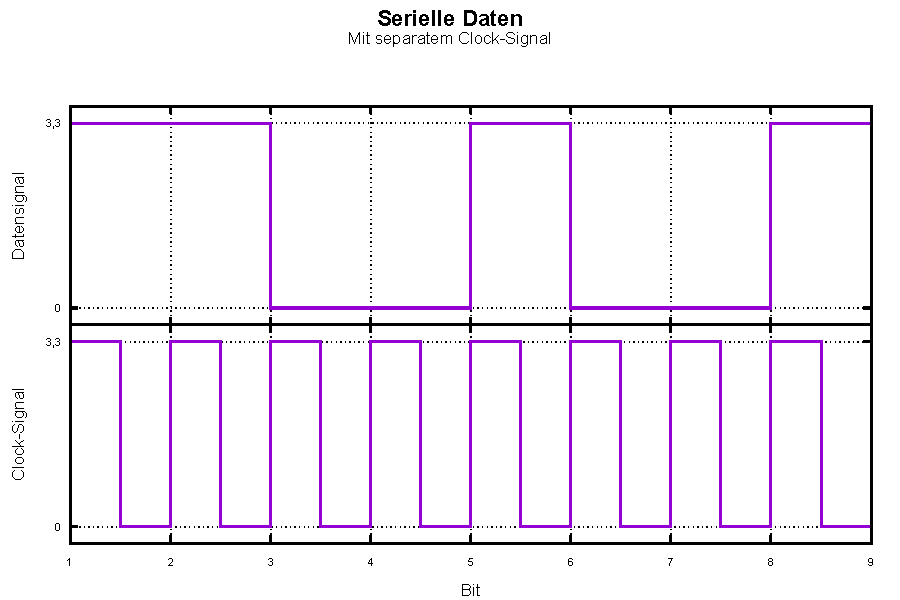
\includegraphics[width=\textwidth]{img/strom-serial} \\
    \end{columns}
\end{frame}


%%% Folie
{
    \setbeamertemplate{background canvas}{
        \includegraphics[height=\paperheight, width=\paperwidth]{img/bauteile}
    }

    \begin{frame}[plain]
    \end{frame}
}

%%% Folie
{
\small

\begin{frame}{Beispiel: Elementare Bauteile}
    \begin{columns}
        \column[b]{.25\textwidth}
        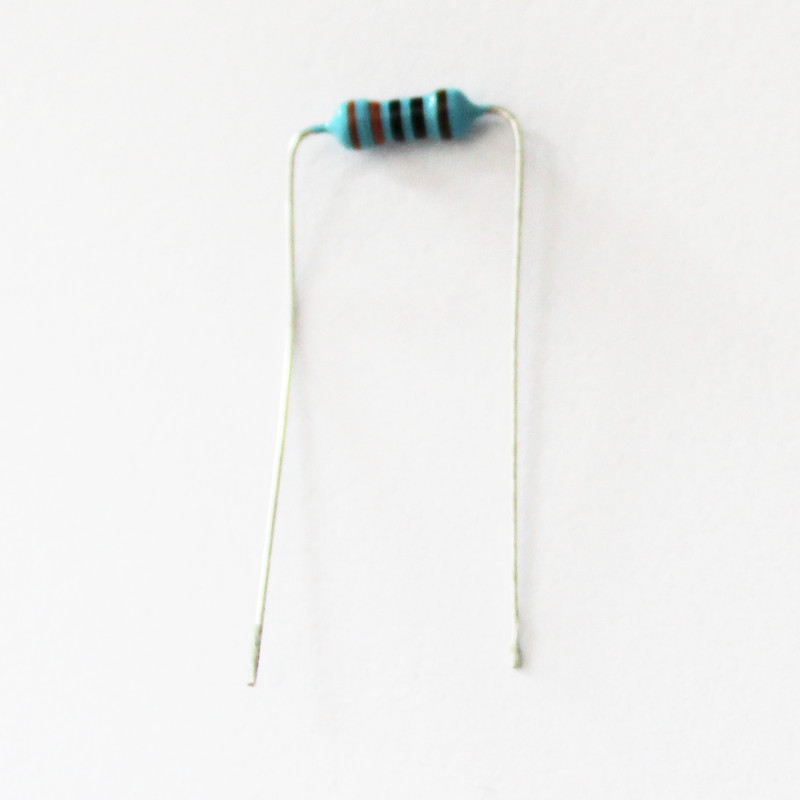
\includegraphics[width=.8\textwidth]{img/komponenten_elementar_widerstand} \\
        Widerstand

        \column[b]{.25\textwidth}
        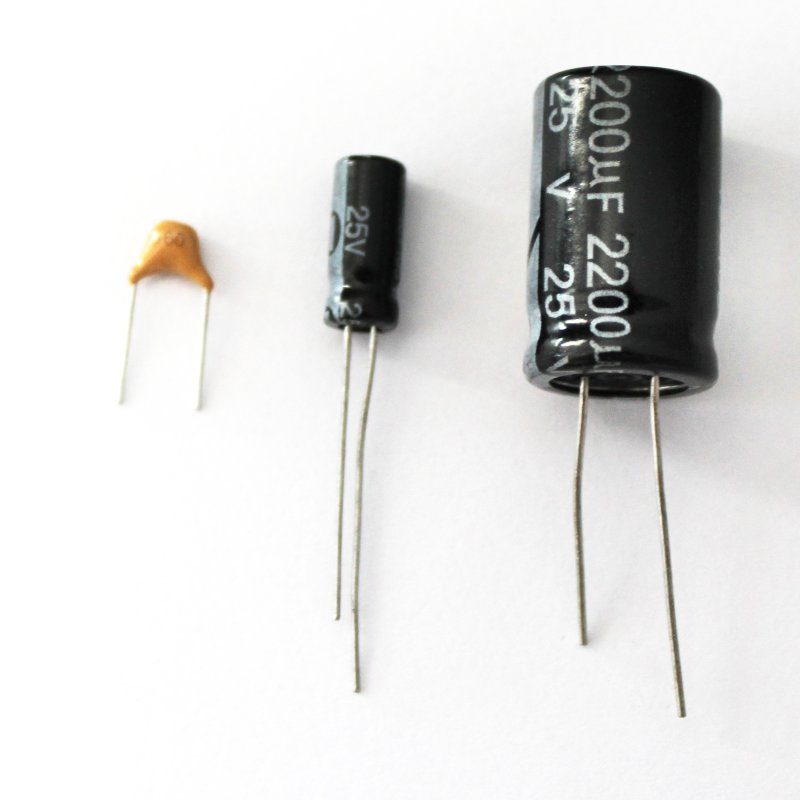
\includegraphics[width=.8\textwidth]{img/komponenten_elementar_kondensator} \\
        Kondensator

        \column[b]{.25\textwidth}
        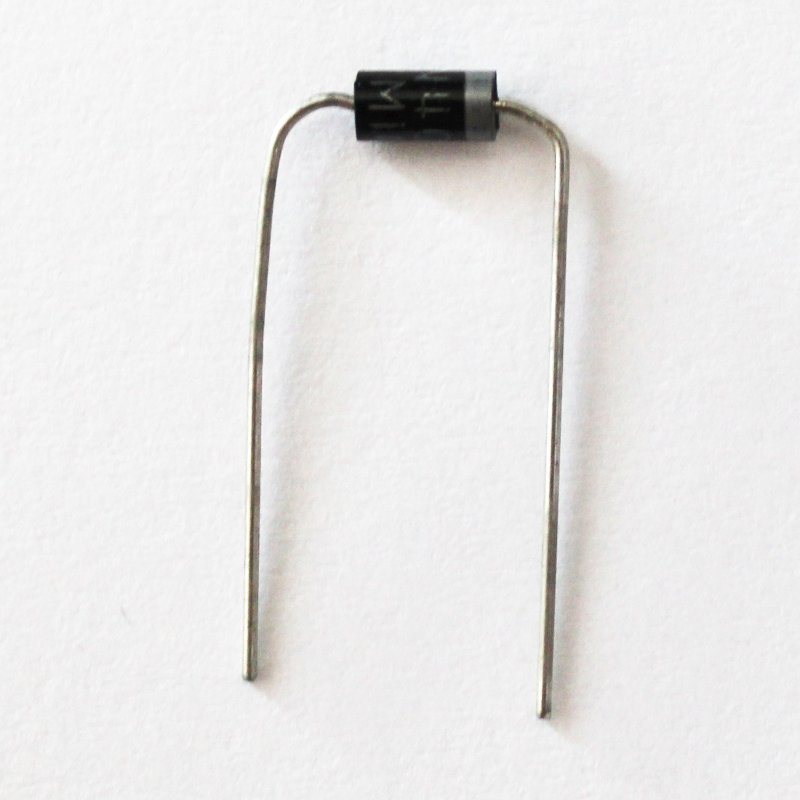
\includegraphics[width=.8\textwidth]{img/komponenten_elementar_diode} \\
        Diode

        \column[b]{.25\textwidth}
        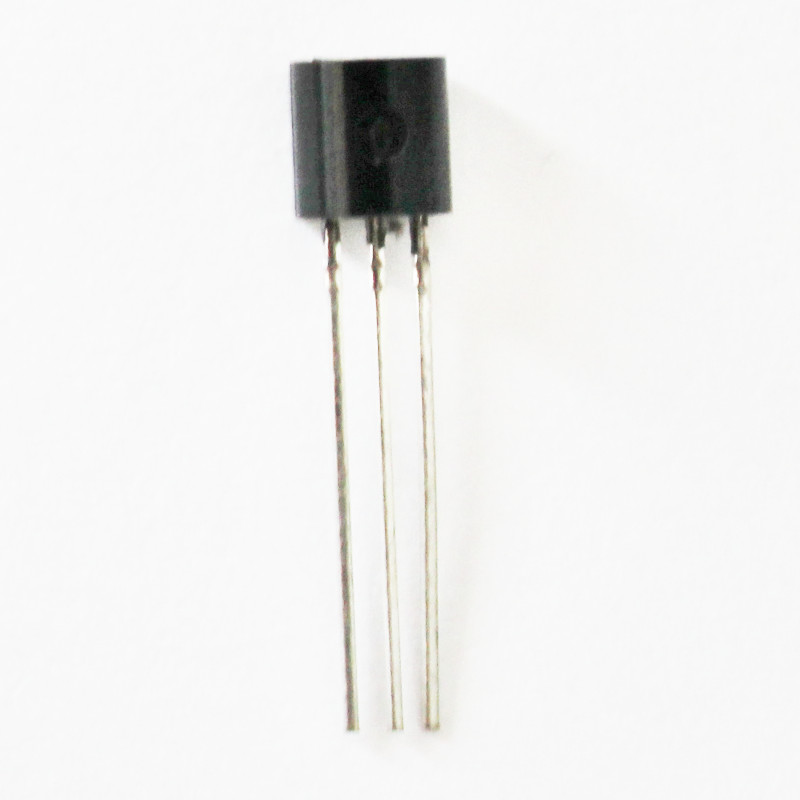
\includegraphics[width=.8\textwidth]{img/komponenten_elementar_transistor} \\
        Transistor
    \end{columns}

    \bigskip

    \begin{columns}
        \column[b]{.25\textwidth}
        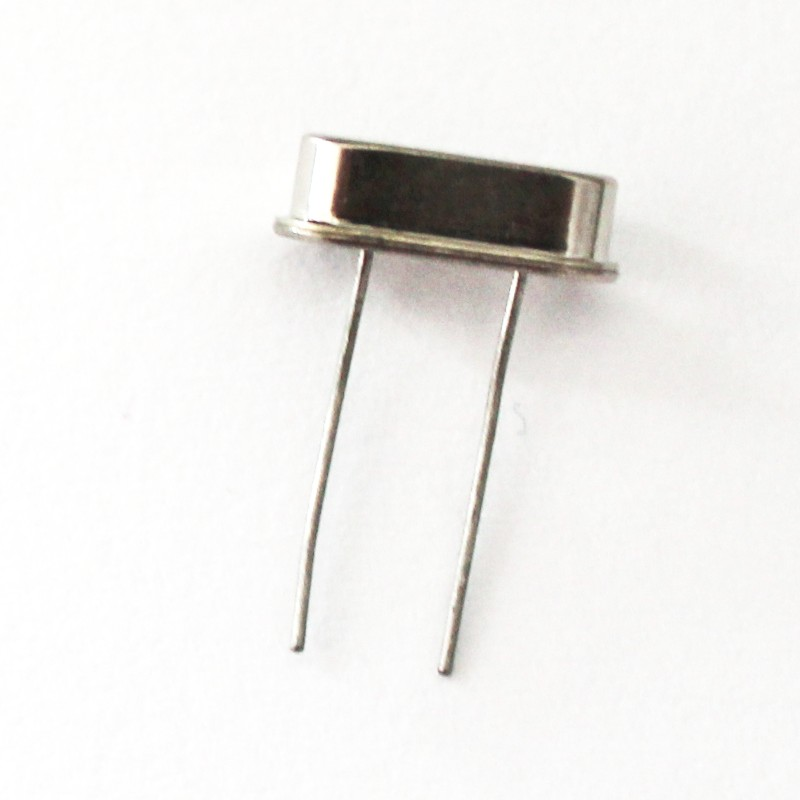
\includegraphics[width=.8\textwidth]{img/komponenten_elementar_quartz} \\
        Quartz-Kristal

        \column[b]{.25\textwidth}
        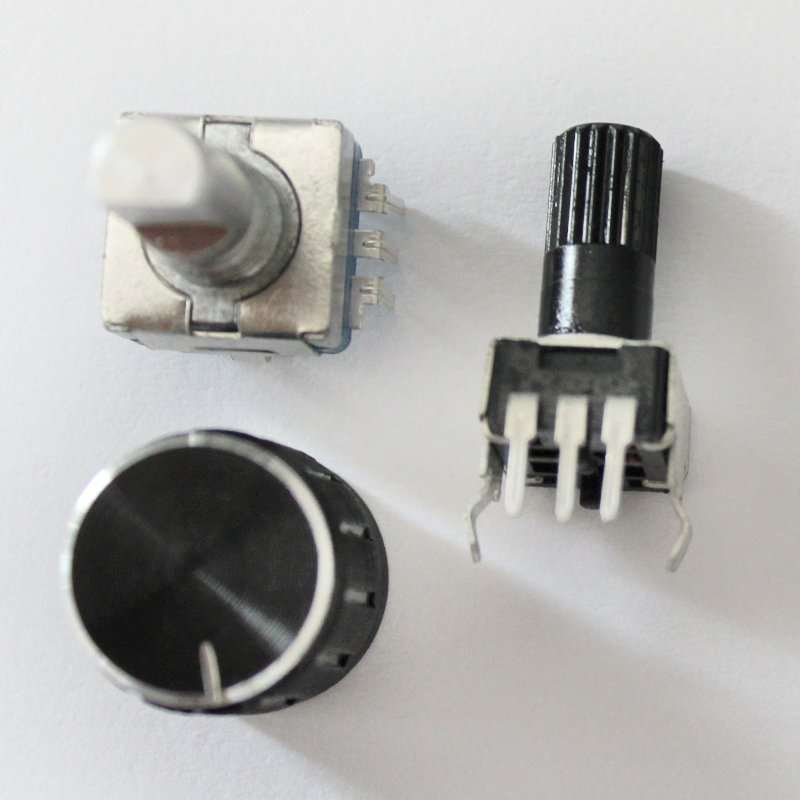
\includegraphics[width=.8\textwidth]{img/komponenten_elementar_drehregler} \\
        Drehregler

        \column[b]{.25\textwidth}
        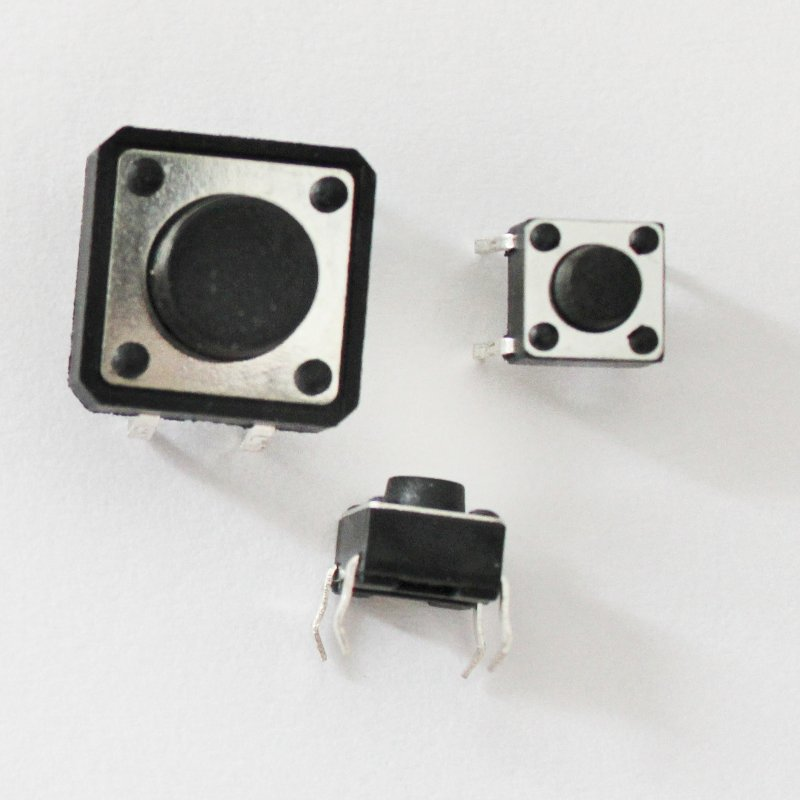
\includegraphics[width=.8\textwidth]{img/komponenten_elementar_taster} \\
        Taster, Schalter

        \column[b]{.25\textwidth}
        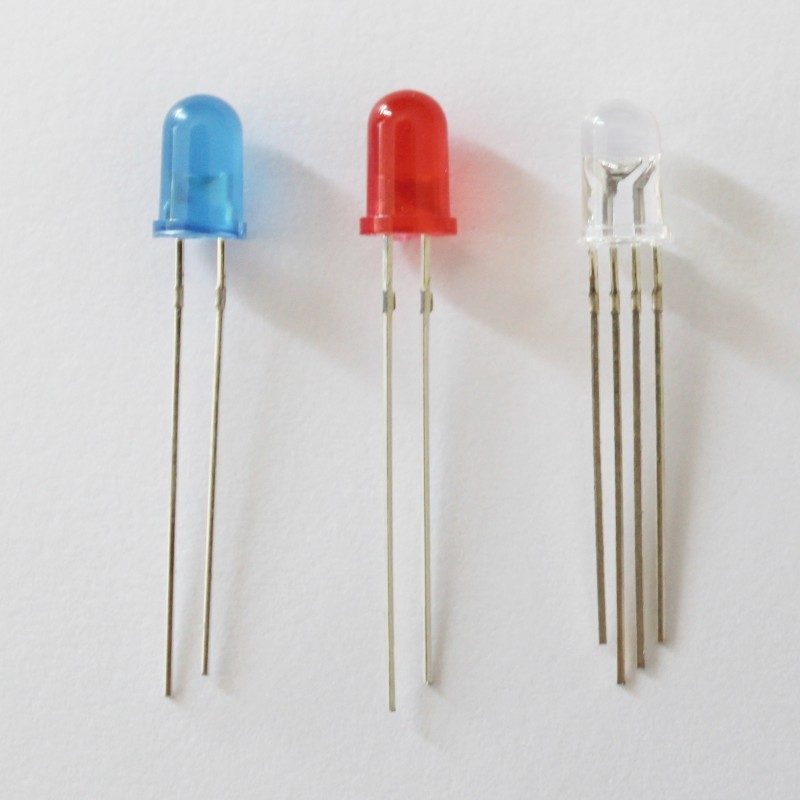
\includegraphics[width=.8\textwidth]{img/komponenten_elementar_led} \\
        Leuchtdiode
    \end{columns}
\end{frame}
}

%%% Folie
{
\tiny

\begin{frame}[allowframebreaks]{Beispiel: DIY-Sensorkit}
    \begin{columns}
        \column{\dimexpr\paperwidth-28pt}
        \begin{center}
            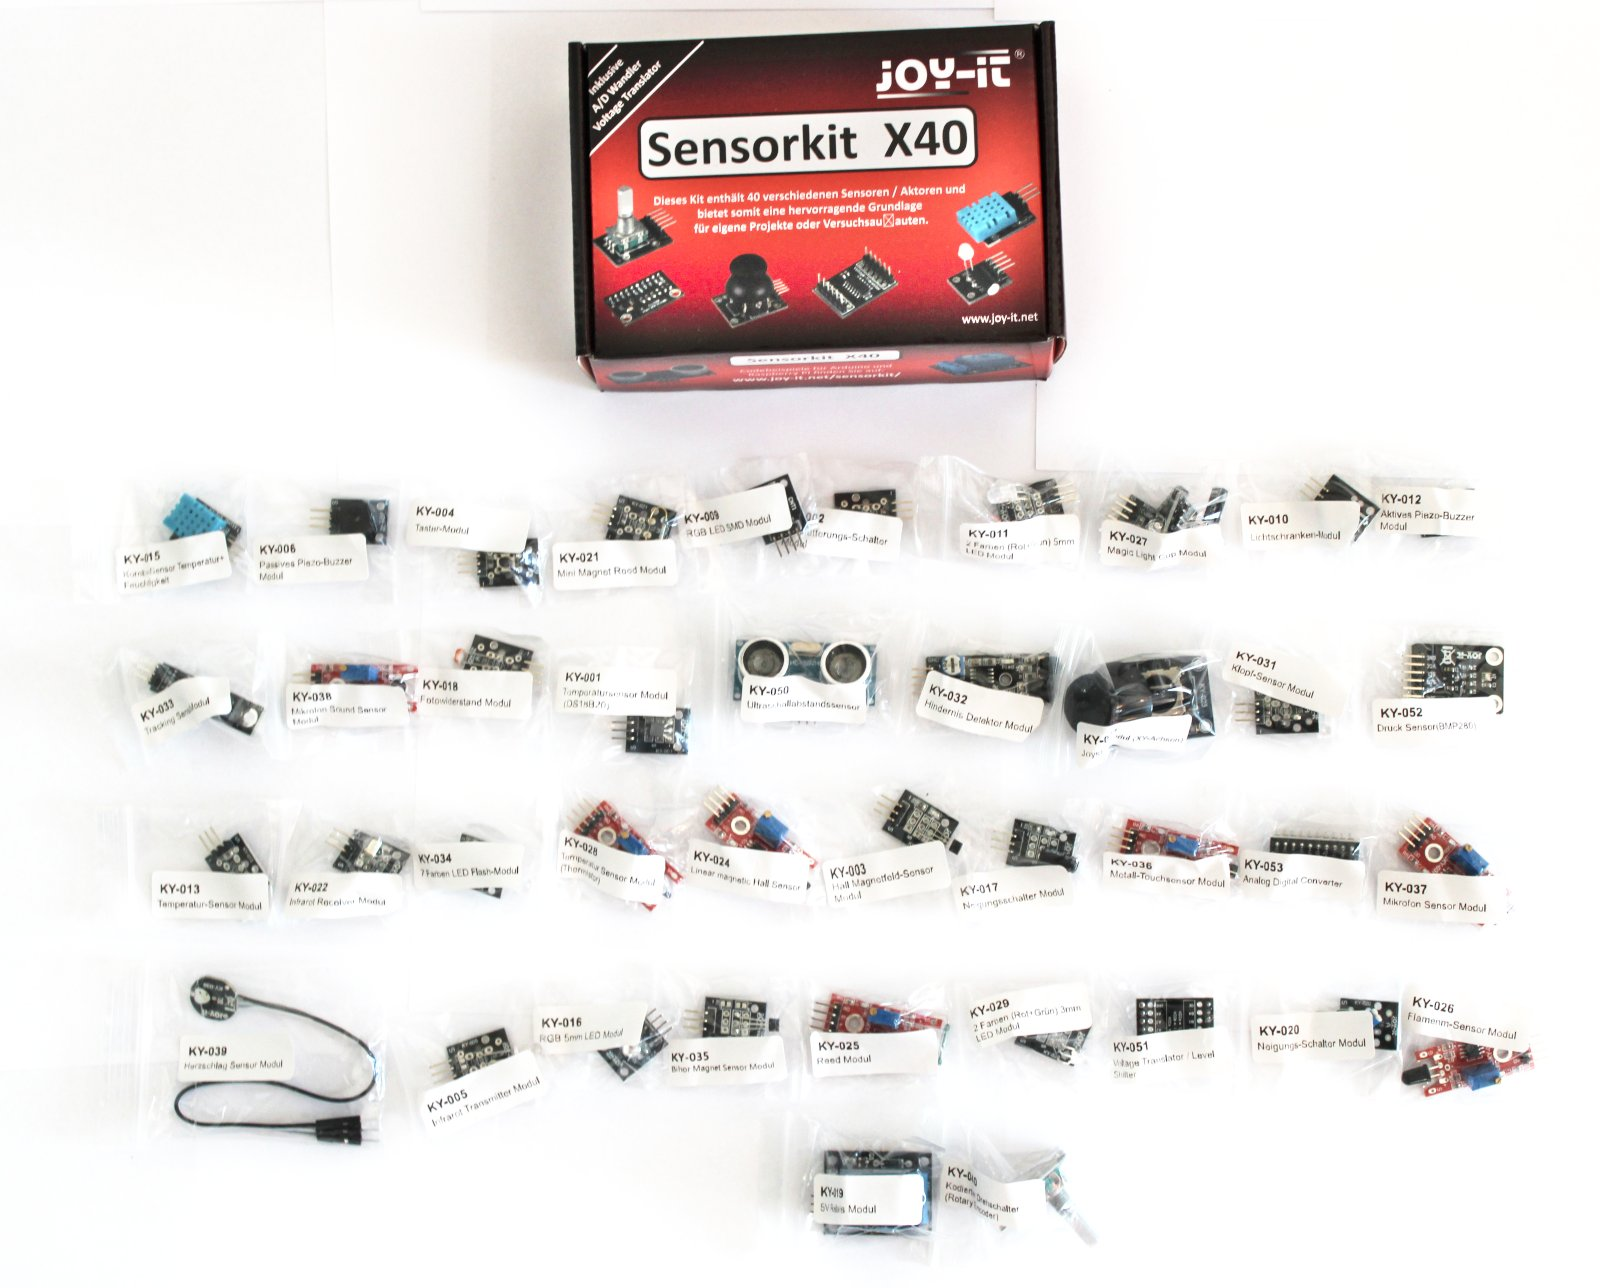
\includegraphics[height=.8\textheight]{img/sensorkit_alle}
        \end{center}
    \end{columns}

    \begin{block}{Umweltsensoren}
        \medskip
        \begin{columns}
            \column{0.5\textwidth}
            KY-001: Temperatursensor (DS18B20) \\
            KY-002: Erschütterungsschalter \\
            KY-003: Hall Magnetfeldsensor \\
            KY-010: Lichtschranke \\
            KY-013: Temperatursensor \\
            KY-015: Temperatur, Feuchtigkeit (DHT11) \\
            KY-017: Neigungsschalter \\
            KY-018: Fotowiderstand \\
            KY-020: Neigungsschalter \\
            KY-021: Mini Magnet-Reedkontakt \\
            KY-024: Linear Magnetic Hall-Sensor \\
            KY-025: Reedkontakt \\
            KY-026: Flammensensor \\

            \column{0.5\textwidth}
            KY-027: Magic Light Cup  \\
            KY-028: Temperatursensor (Thermistor) \\
            KY-031: Klopfsensor \\
            KY-032: Hindernisdetektor \\
            KY-033: Trackingsensor \\
            KY-035: Bihor Magnetsensor \\
            KY-036: Metall-Touchsensor \\
            KY-037: Mikrofon Soundsensor \\
            KY-038: Mikrofon Soundsensor \\
            KY-039: Herzschlagsensor \\
            KY-050: Ultraschallabstandssensor \\
            KY-052: Drucksensor (BMP280) \\
        \end{columns}
    \end{block}

    \begin{block}{Ein-/Ausgabemodule}
        \medskip
        \begin{columns}
            \column{0.5\textwidth}
            KY-004: Taster \\
            KY-022: Infrarot-Receiver \\
            KY-023: XY-Joystick \\
            KY-040: Kodierter Drehschalter (Rotary Encoder) \\
            \smallskip
            KY-005: Infrarot-Transmitter \\
            KY-006: Passiver Piezo-Buzzer \\
            KY-009: RGB-LED (Surface-Mount) \\

            \column{0.5\textwidth}
            KY-011: 2-Farben (Rot und Grün) LED \\
            KY-012: Aktiver Piezo-Buzzer \\
            KY-016: RGB-LED (Through-Hole) \\
            KY-019: 5V Relais \\
            KY-029: 2-Farben (Rot und Grün) LED \\
            KY-034: 7-Farben LED \\
        \end{columns}
    \end{block}

    \begin{block}{Hilfsbausteine}
        \medskip
        \begin{columns}
            \column{0.5\textwidth}
            KY-051: Voltage Translator / Level Shifter \\

            \column{0.5\textwidth}
            KY-053: Analog/Digital Converter \\
        \end{columns}
    \end{block}
\end{frame}
}

%%% Folie
{
\small

\begin{frame}{Beispiel: Integrierte Schaltkreise}
    \begin{columns}
        \column[b]{.5\textwidth}
        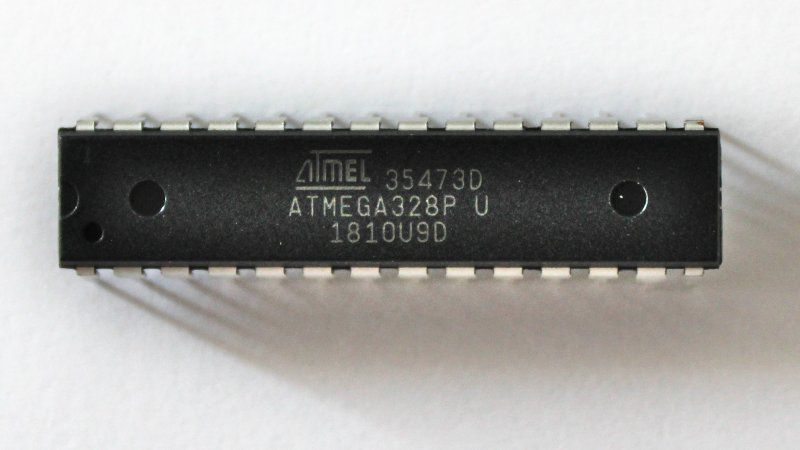
\includegraphics[width=.8\textwidth]{img/komponenten_ic_prozessor} \\
        Mikroprozessor, Mikrocontroller

        \column[b]{.5\textwidth}
        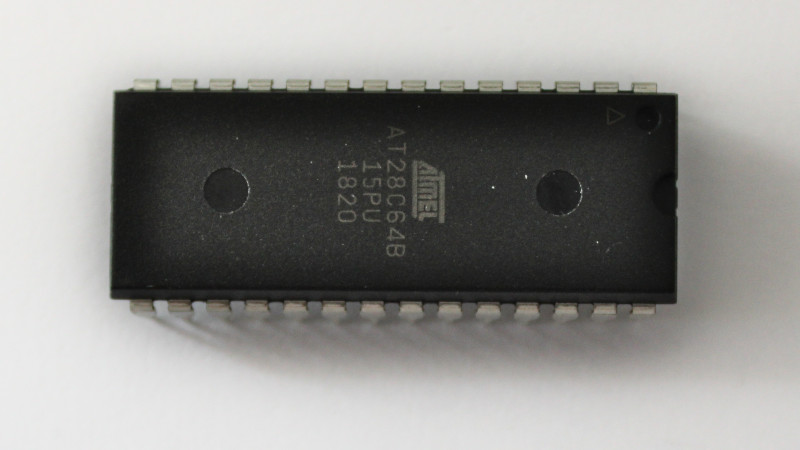
\includegraphics[width=.8\textwidth]{img/komponenten_ic_speicher} \\
        Speicherbaustein
    \end{columns}

    \bigskip

    \begin{columns}
        \column[b]{.5\textwidth}
        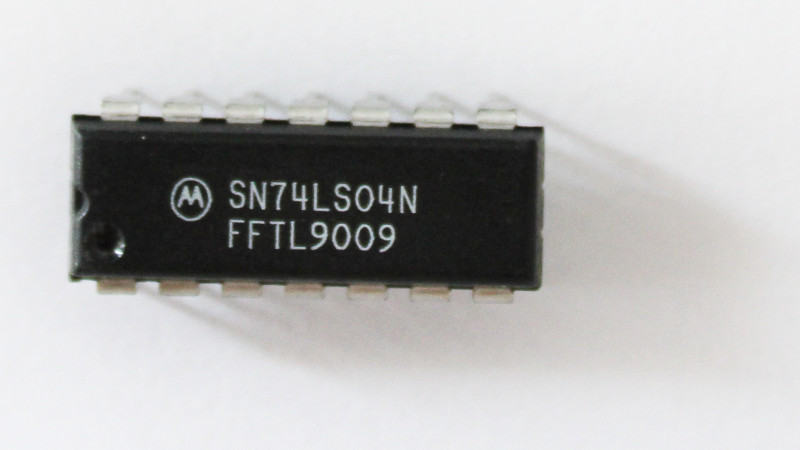
\includegraphics[width=.8\textwidth]{img/komponenten_ic_logikgatter} \\
        Logikbaustein (AND, OR, XOR, ...)

        \column[b]{.5\textwidth}
        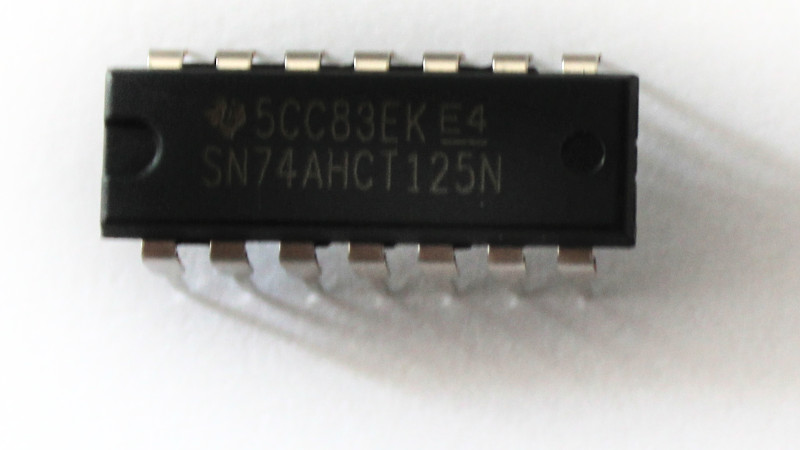
\includegraphics[width=.8\textwidth]{img/komponenten_ic_levelshifter} \\
        Level Shifter
    \end{columns}

    \bigskip

    \textbf{Häufig verwendet:} A/D-Wandler, D/A-Wandler, PWM-Treiber, GPIO-Extender, \ldots
\end{frame}
}

%%% Folie
{
\small

\begin{frame}{Beispiel: Vorgefertigte Baugruppen}
    \begin{columns}
        \column[b]{.5\textwidth}
        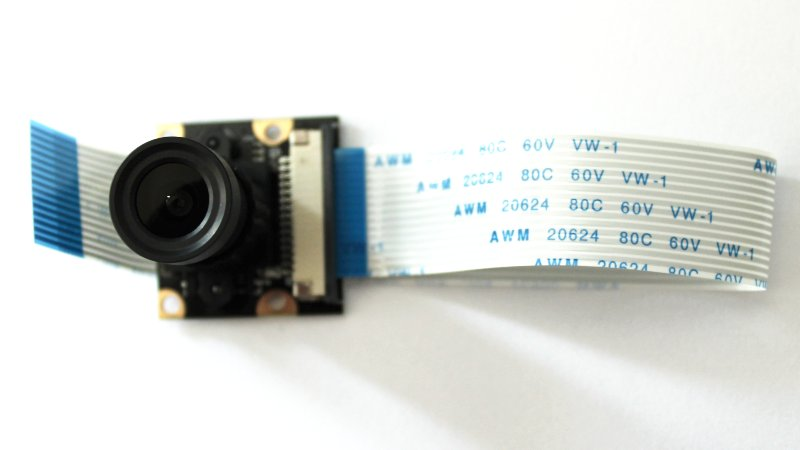
\includegraphics[width=.8\textwidth]{img/komponenten_baugruppen_kamera} \\
        Kameramodul

        \column[b]{.5\textwidth}
        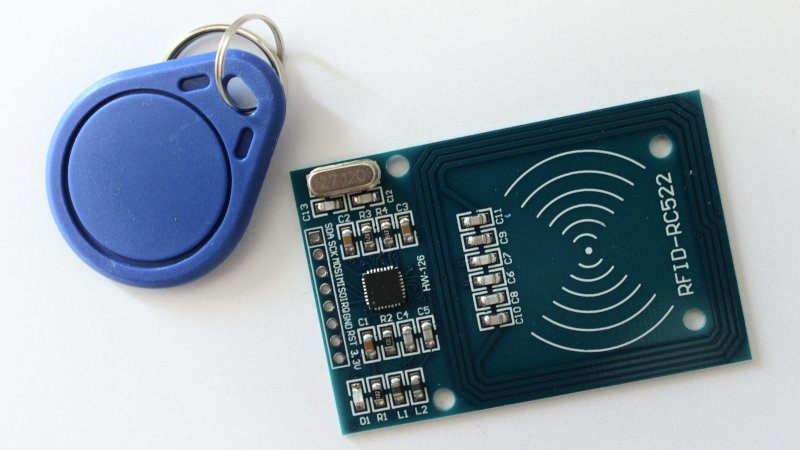
\includegraphics[width=.8\textwidth]{img/komponenten_baugruppen_rfid} \\
        RFID-Leser
    \end{columns}

    \bigskip

    \begin{columns}
        \column[b]{.5\textwidth}
        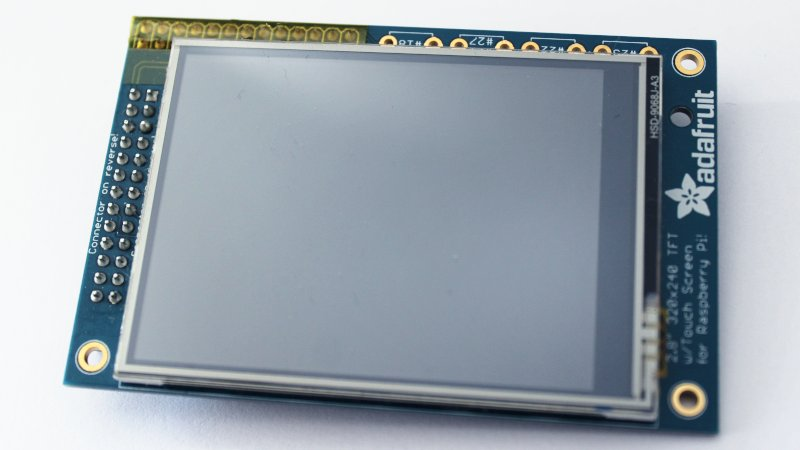
\includegraphics[width=.8\textwidth]{img/komponenten_baugruppen_display} \\
        Display

        \column[b]{.5\textwidth}
        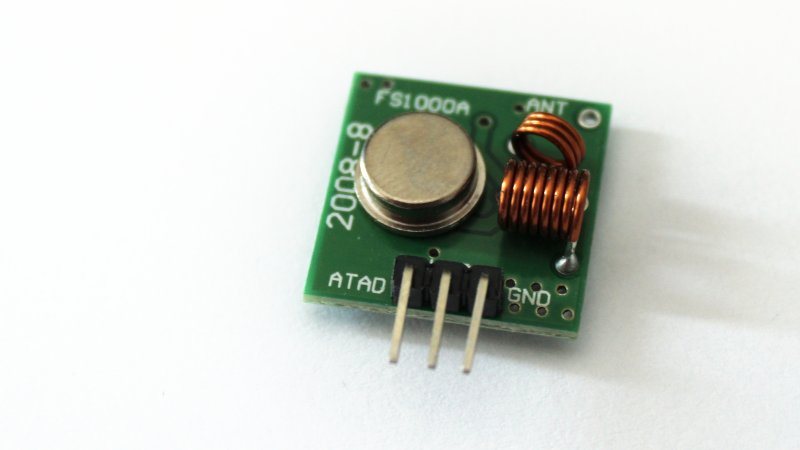
\includegraphics[width=.8\textwidth]{img/komponenten_baugruppen_funk} \\
        Funkmodul
    \end{columns}
\end{frame}
}

%%% Folie
{
\small

\begin{frame}{Beispiel: Modular einsetzbare Geräte}
    \begin{columns}
        \column[b]{.5\textwidth}
        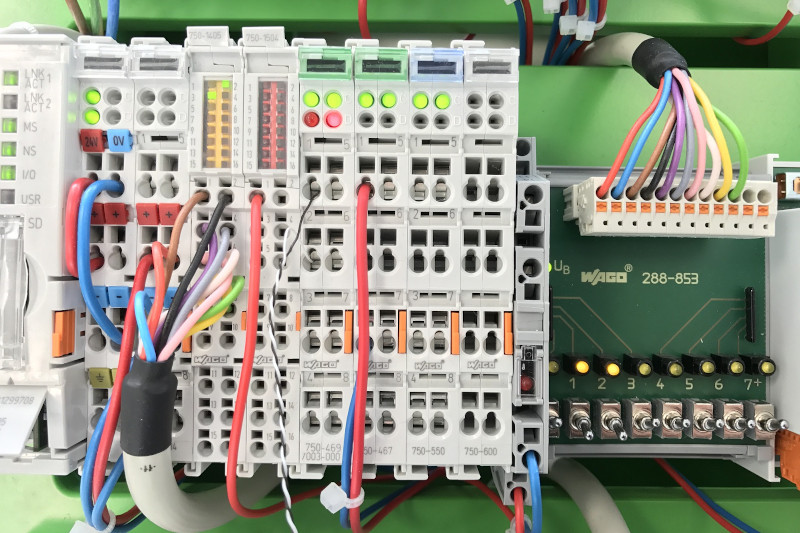
\includegraphics[width=.8\textwidth]{img/komponenten_geraete_industriesteuerung} \\
        Industrielle Steuergeräte

        \column[b]{.5\textwidth}
        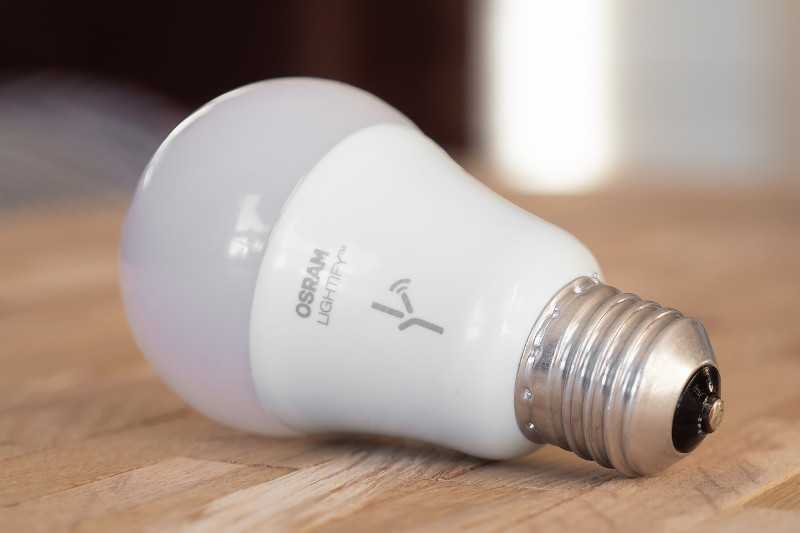
\includegraphics[width=.8\textwidth]{img/komponenten_geraete_smarthome} \\
        Smart-Home-Komponenten
    \end{columns}

    \bigskip

    \begin{columns}
        \column[b]{.5\textwidth}
        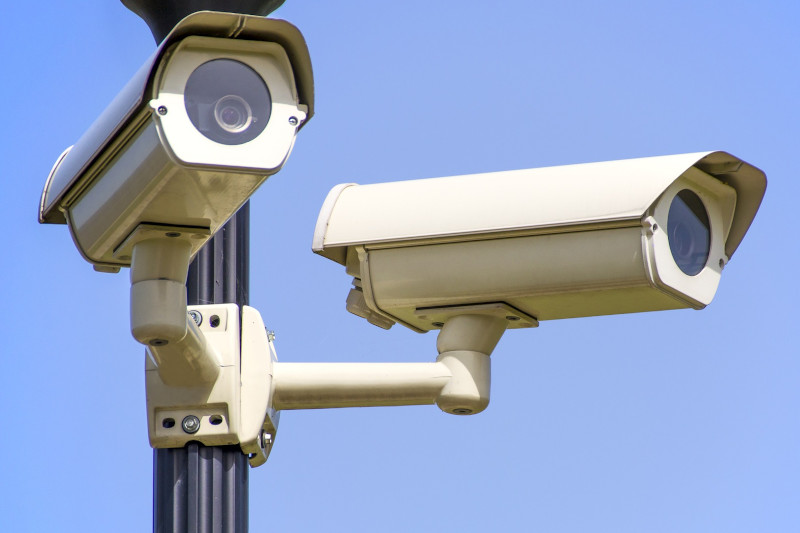
\includegraphics[width=.8\textwidth]{img/komponenten_geraete_ipkamera} \\
        IP-Kameras

        \column[b]{.5\textwidth}
        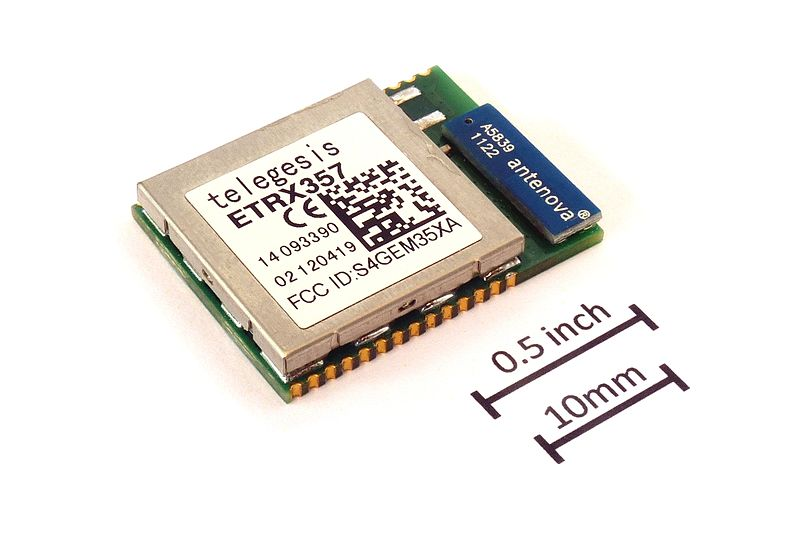
\includegraphics[width=.8\textwidth]{img/komponenten_geraete_zigbee} \\
        ZigBee-Sensoren und Aktoren
    \end{columns}
\end{frame}
}

%%% Folie
{
    \setbeamertemplate{background canvas}{
        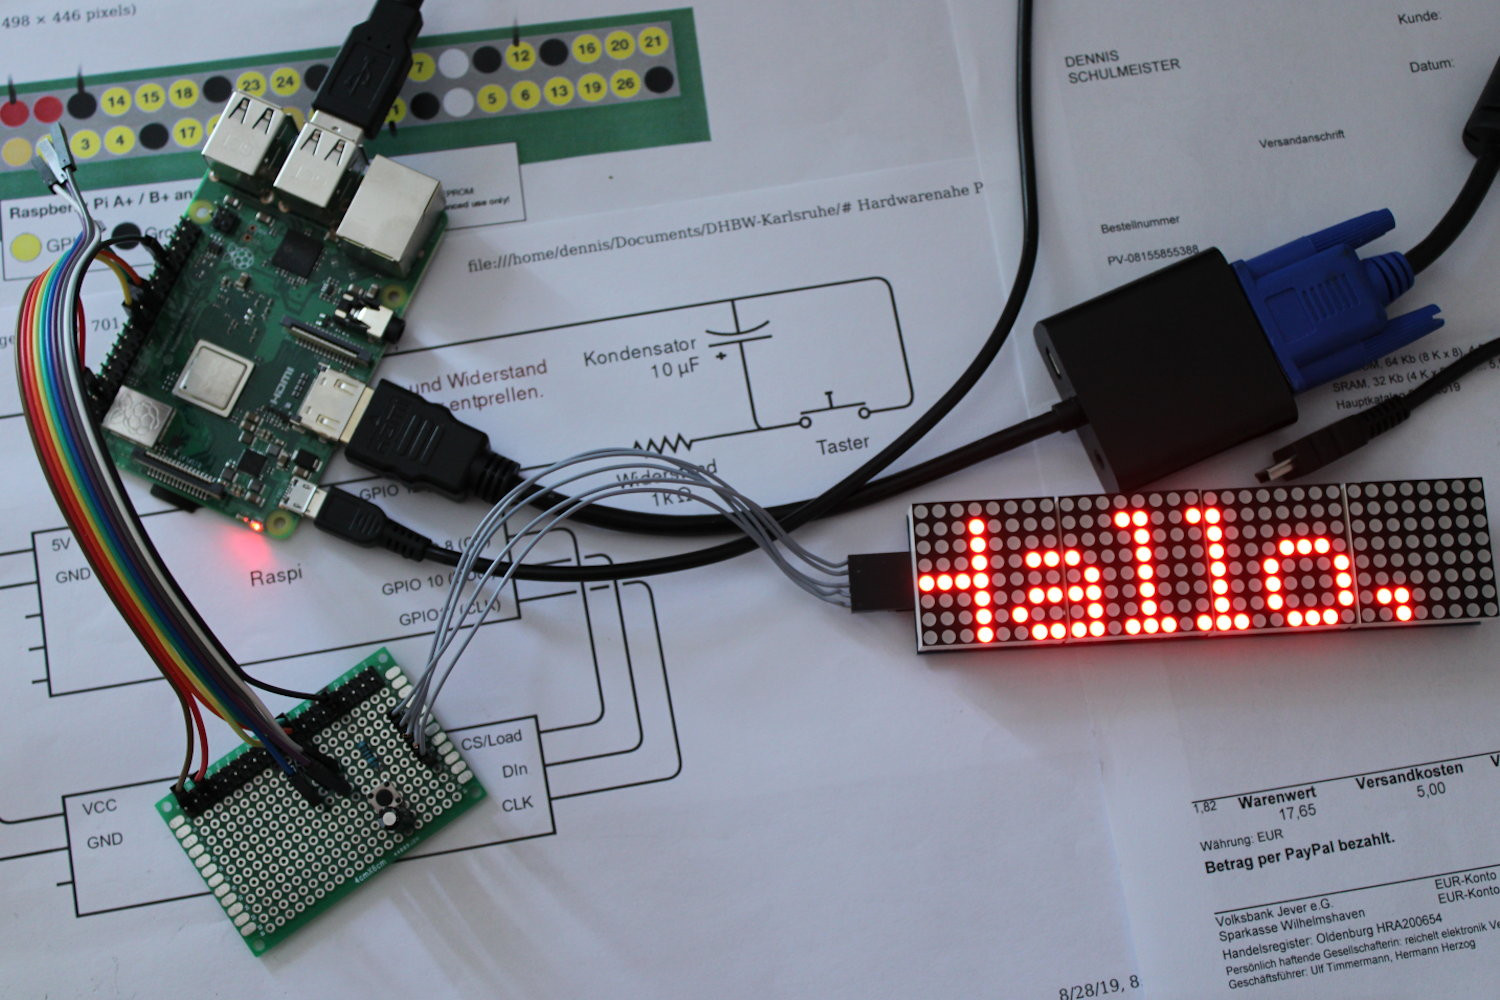
\includegraphics[height=\paperheight, width=\paperwidth]{img/vorgehen_lochrasterplatine}
    }

    \begin{frame}[plain]
    \end{frame}
}

%%% Folie
{
    \setbeamertemplate{background canvas}{
        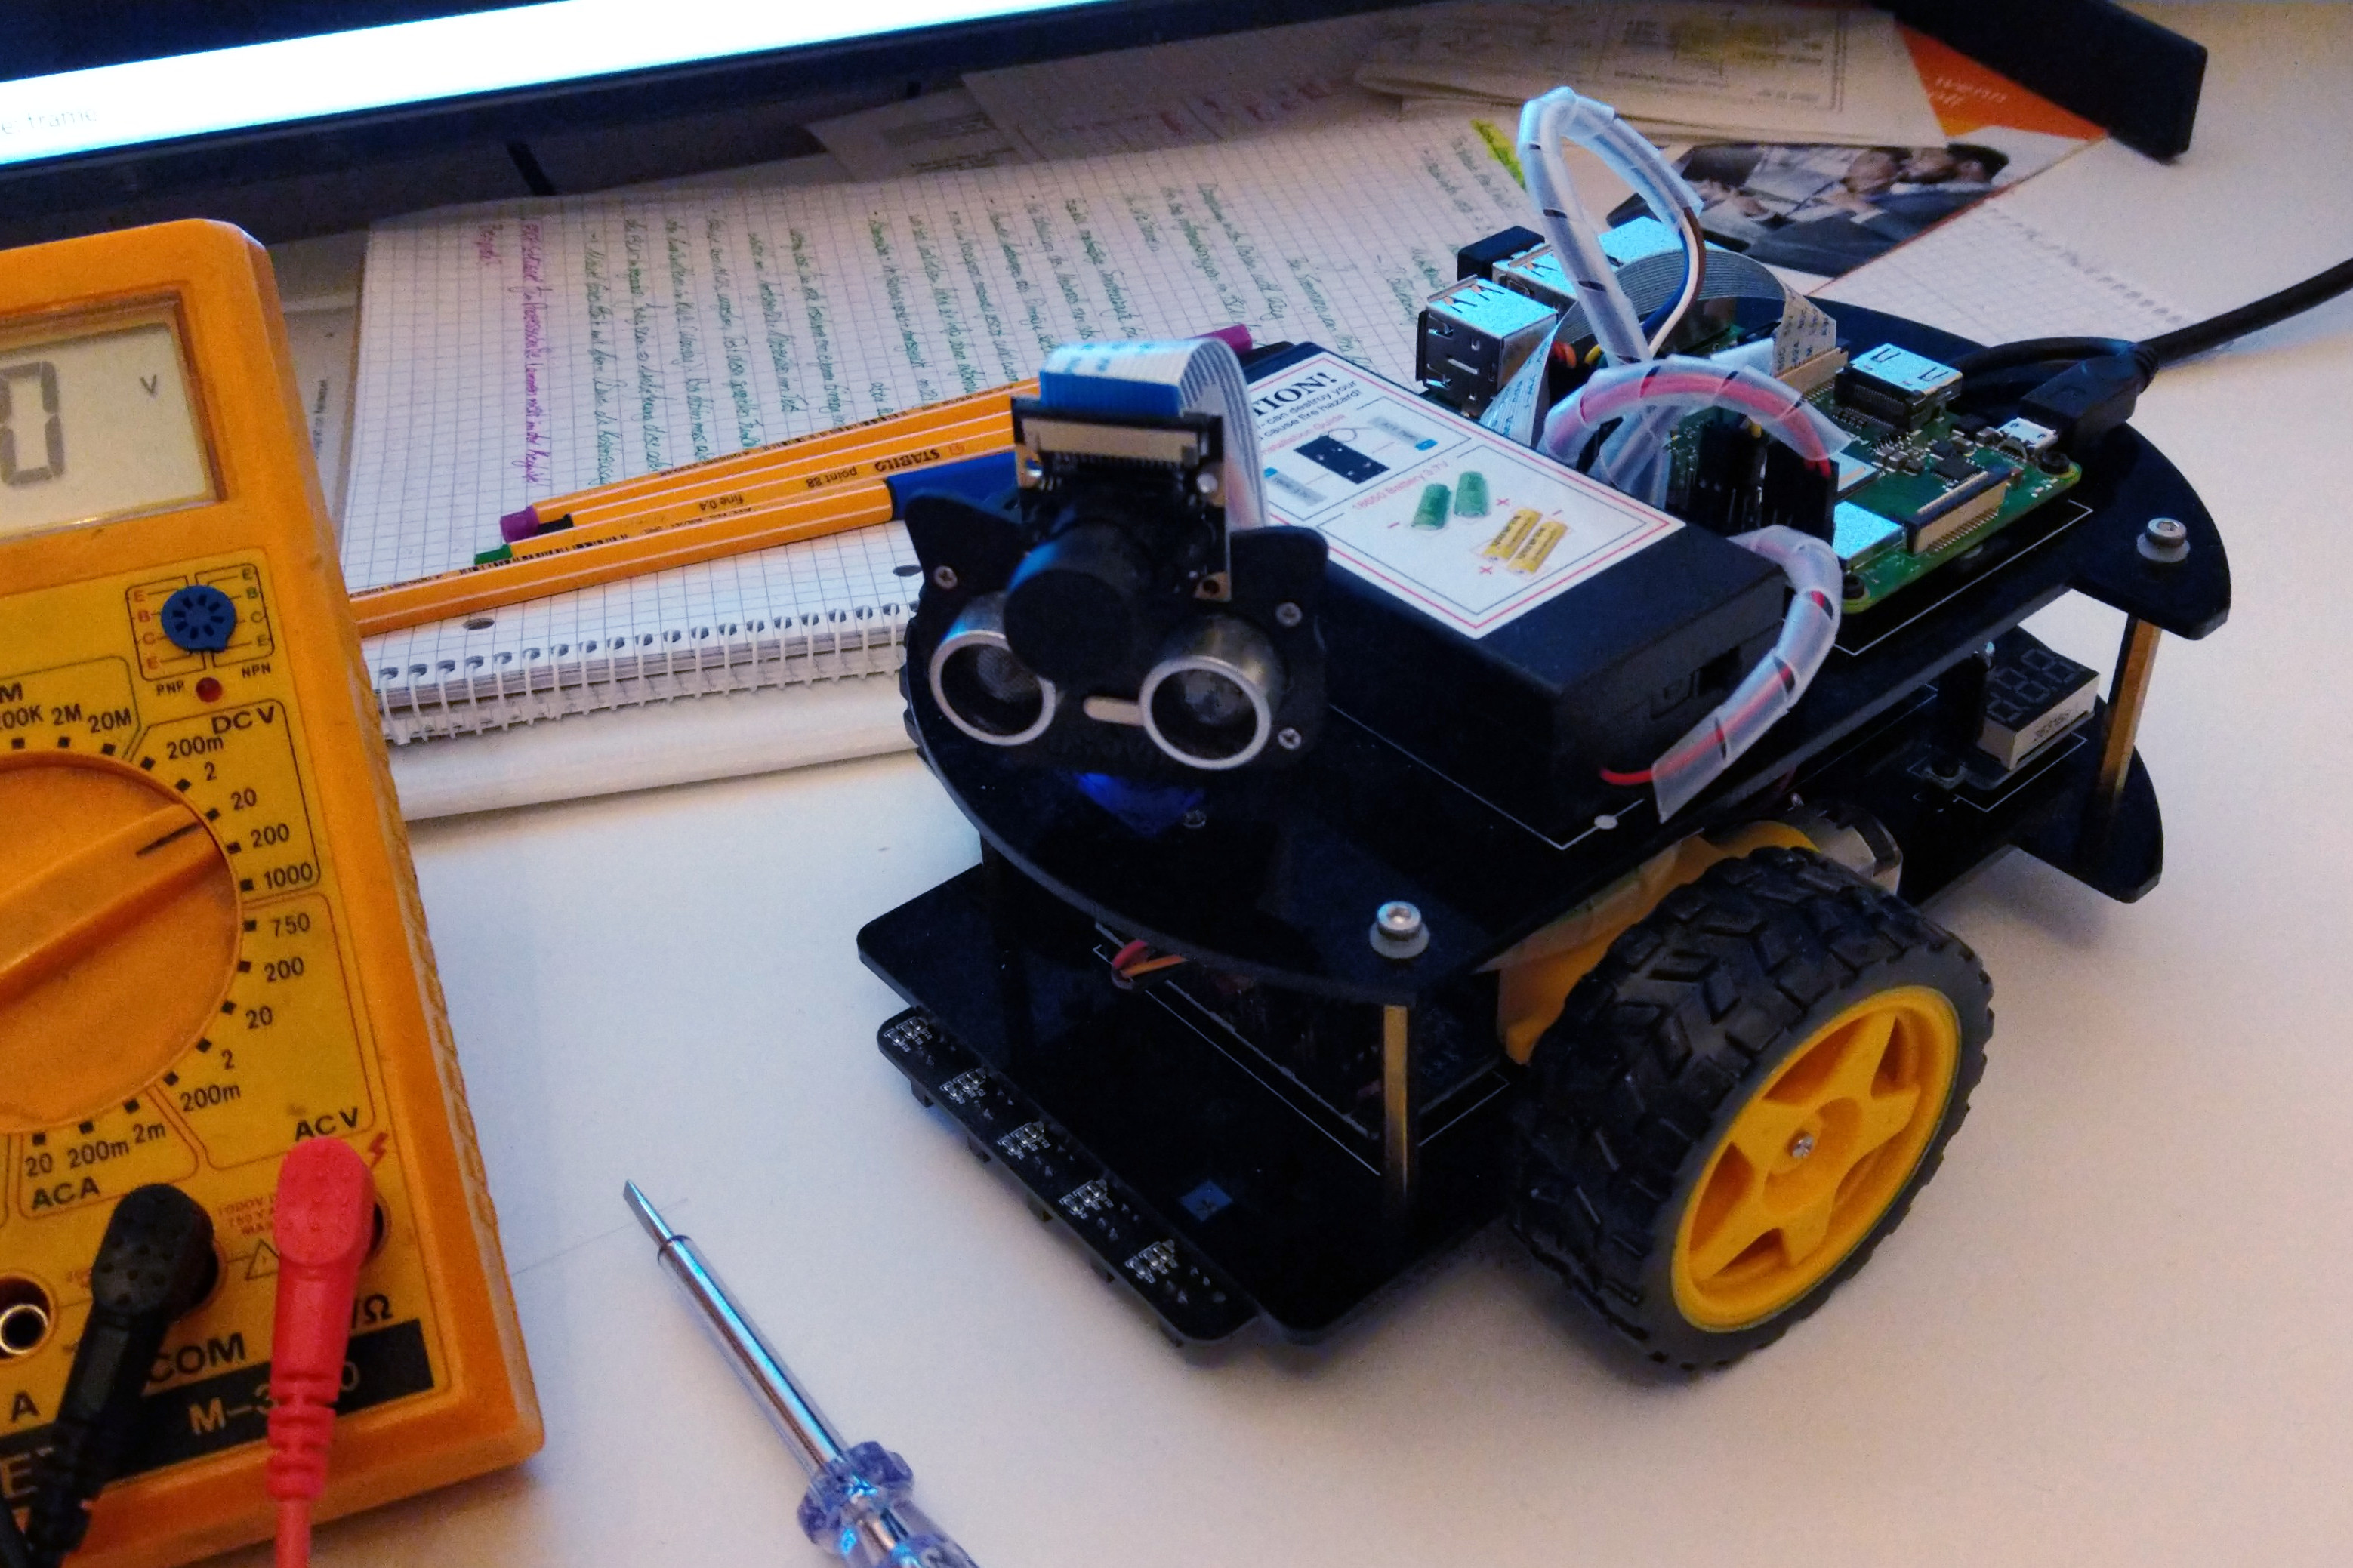
\includegraphics[height=\paperheight, width=\paperwidth]{img/fallbeispiel_fahrzeug}
    }

    \begin{frame}[plain]
    \end{frame}
}

%-------------------------------------------------------------------------------
\section{Typische Grundschaltungen}
%-------------------------------------------------------------------------------

%%% Folie
{
\scriptsize

\begin{frame}{Den Raspberry Pi mit Strom versorgen}
    \begin{columns}
        \column{.5\textwidth}
        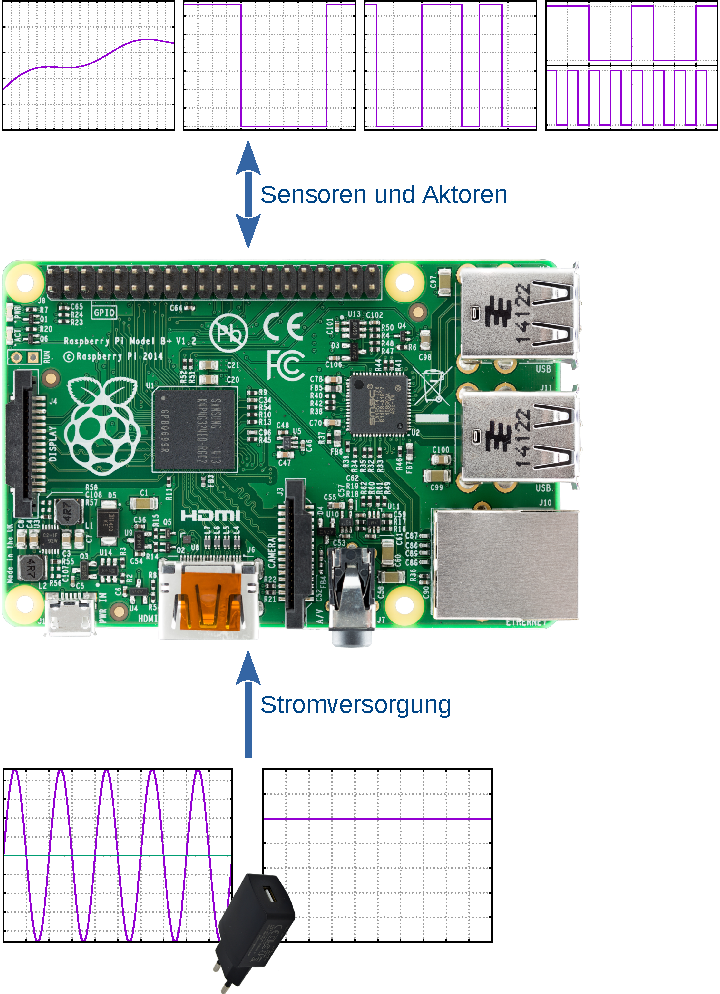
\includegraphics[width=\textwidth]{img/raspi-stromarten}

        \column{.5\textwidth}

        \begin{block}{Stromversorgung}
            \smallskip
            \parbox{\linewidth}{
                Das Stromnetz liefert Wechselstrom mit 230\,V und 16\,A.
                Der Raspberry Pi benötigt aber \textbf{5\,V Gleichstrom und $\pm$ 3\,A}.
                Das Netzteil muss daher den die Spannung reduzieren und den Strom gleichrichten.
                Eine mobile Stromversorgung muss mindestens genauso viel Strom liefern.
                \smallskip

                \textcolor{red}{
                    Die Spannung muss dabei möglichst konstant sein und darf nicht
                    überschritten werden, um Beschädigungen zu vermeiden!
                }
            }
        \end{block}

        \vfill

        \begin{block}{Batterielaufzeit}
            \smallskip
            \parbox{\linewidth}{
                Kann über die Nennladung der Batterie abgeschätzt werden, wenn diese
                bekannt ist:
                \smallskip

                $\text{Laufzeit in Stunden} = \frac{\text{Nennladung in Ah}}{\text{Stromverbrauch in A}}$
            }
        \end{block}

        \vfill

        \begin{block}{Stromkosten}
            \smallskip
            \parbox{\linewidth}{
                Kann durch Umrechnen des Stromverbrauchs in Killowatt berechnet werden:
                \smallskip

                $\text{Kosten} = \frac{5\,V \times 3\,A}{1000} \times \text{Stunden} \times \text{Strompreis je kWh}$
            }
        \end{block}
    \end{columns}
\end{frame}
}

%%% Folie
{
\footnotesize

\begin{frame}{Maximale Grenzwerte}
    \parbox{\linewidth}{
        Um eine Beschädigung des Raspberry Pi zu vermeiden, müssen folgende Grenzwerte unbedingt
        eingehalten werden. Ggf. müssen daher Widerstände in Serie zu einem Bauteil angeschlossen
        werden, um die Stromstärke zu begrenzen. Ebenso muss die Summe aller zugeführten und entnommenen
        Ströme betrachtet werden.
    }

    \bigskip
    \renewcommand{\arraystretch}{1.2}

    \begin{tabularx}{\textwidth}{|p{18em}|X|X|}
        \hline
        \textbf{Parameter} & \textbf{Mindestwert} & \textbf{Maximalwert} \\
        \hline

        Betriebsspannung des Pi & 5\,V & 5\,V \\
        \hline

        Stromverbrauch des Pi & 800\,mA (eher mehr) & -- \\
        \hline

        Stromentnahme an den 3.3\,V-Pins & -- & 50\,mA gesamt \\
        \hline

        Stromentnahme an den 5\,V-Pins & -- & 50\,mA gesamt \\
        \hline

        Stromentnahme an einem GPIO-Pin & -- & 16\,mA \\
        \hline

        Stromentnahme an allen GPIO-Pins & -- & 50\,mA gesamt \\
        \hline
    \end{tabularx}

    \bigskip
    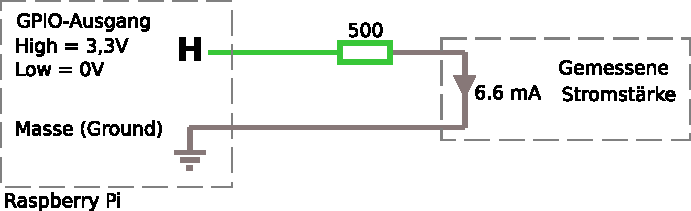
\includegraphics[width=.75\textwidth]{img/stromentnahme-raspi-schaltplan}

    \hfill%
    \CircuitJS{https://www.falstad.com/circuit/circuitjs.html?ctz=CQAgzCAMB0l3BWEBGGAmOaDsWyQBxoBsAnCViApJZdQgKYC0yyAUADIj7JEhr74QWIoP6DqyEADMAhgBsAzvXDQIkVmCzUSAFh18BIXfrBhek6uoDmQkeDO3BYBGihRWAJy48Dg477cqdQAjIRIkNAQkIh0KTX11AHcjPXteYScHdQAPEBiScHwKLDQTEmp9ZFcAJRkFAAdg+g8PAE8AHQUABQBLVlyiBApsVywdCGwkStcAcS6ASQB5RgBBAFcFKxkAOyt+vIReMB1JLCpwVOmQAFk6pU6AChmPAHs17YATAEp9waPICBYZAQPC8K7sF6JTrtACOnUgADVfocAiVRCRJFcABI9KwAC2hcIUYAANGAkblUJATJBXKgxuBIFMULN6ABbegKJTbej7KlHZAFekFMBoVxXADKABdXmyFFKACceADWvNCqEMx30JDQBWwBXUQA}
\end{frame}
}

%%% Folie
{
\scriptsize

\begin{frame}{Binärsignal ausgeben am Beispiel einer LED}
    \Justified{
        Jeder \textbf{GPIO-Pin} kann softwaregesteuert als \textbf{Eingang oder Ausgang} konfiguriert
        werden. Ausgangspins stellen eine Spannung von \textbf{ca. 3,3\,V} zur Verfügung, um eine
        logische Eins zu signalisieren, sowie \textbf{0\,V} (entspricht einer Verbindung gegen Masse)
        für eine logische Null.
        \smallskip

        Der entnommene Strom muss in der Regel durch einen \textbf{Widerstand} begrenzt werden.
        Da die verfügbare Spannung und die gewünschte Stromstärke bekannt sind, kann dieser mit
        dem \textbf{Ohmschen Gesetz} leicht berechnet werden. Dabei muss jedoch auch der innere
        Widerstand des angeschlossenen Bauteils, der nicht immer leicht zu ermitteln ist,
        berücksichtigt werden, da dieser den Gesamtwiderstand erhöht und die Strommenge dadurch
        zusätzlich begrenzt.
        \smallskip

        \textcolor{red}{
            Die entnommenen Ströme dürfen nicht größer als 16\,mA und ihre Summe nicht größer als 50\,mA sein.
        }
    }

    \bigskip

    \begin{columns}
        \column{0.5\textwidth}
        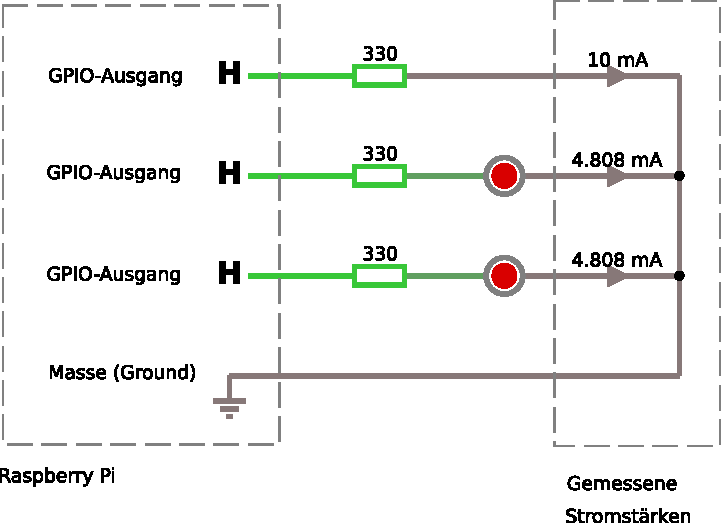
\includegraphics[width=\textwidth]{img/led_direkt_circuitjs}
        \smallskip

        \CircuitJS{https://www.falstad.com/circuit/circuitjs.html?ctz=CQAgjCAMB0l3BWcMBMcUHYMGZIA4UA2ATmIxAUgoqoQFMBaMMAKAHMRCUAWCsFTjwoo8UKCwBOnDAO7dRGQqLmiq2XCzBcQi5fJB5ss-QIAmdAGYBDAK4AbAC4M7dU+DFUYkVgBlpx0S5eFTEIazsAZzoQbGhscT9CGRi8XiCU3iowq0jo2PjISX8MnSUStQ1sDCpDAWxUkGJ+EohPFiqaoxAQpoD3NoB3Rub63l7u-UKh8Z7mhGbCrQFdEtqSs0tbR2dXfo9YVmm55vT5gULE5KMqdOvQkHComLjxKSS6tFLRO4qpr5jPmsfu1qgYundxndWuIjh8qJCGoUAEacBCEECYJDcDDECho8QAD26igoeFo81J8V4zQASlYIgAHJF0CQSACeAB0IgAFACWLCJlG+QgQxF4RnI1IEAHFuQBJADyDAAgjYImwrAA7NgCmiieZpSACeaS8ACACy9KiXIAFNKJAB7Gya0wASl1lHI9XRovi9VxUpAssVKrVGu1Hsgkopvu6CGCZqD8qVqvVWp1KLWmAExHqePIhSJqVoeCQTRLykT0roAFs6BEopq6LrDLjCJB0U025AA4mAMoOR01iIOAAnEgA1nRNSwgA}

        \column{0.5\textwidth}
        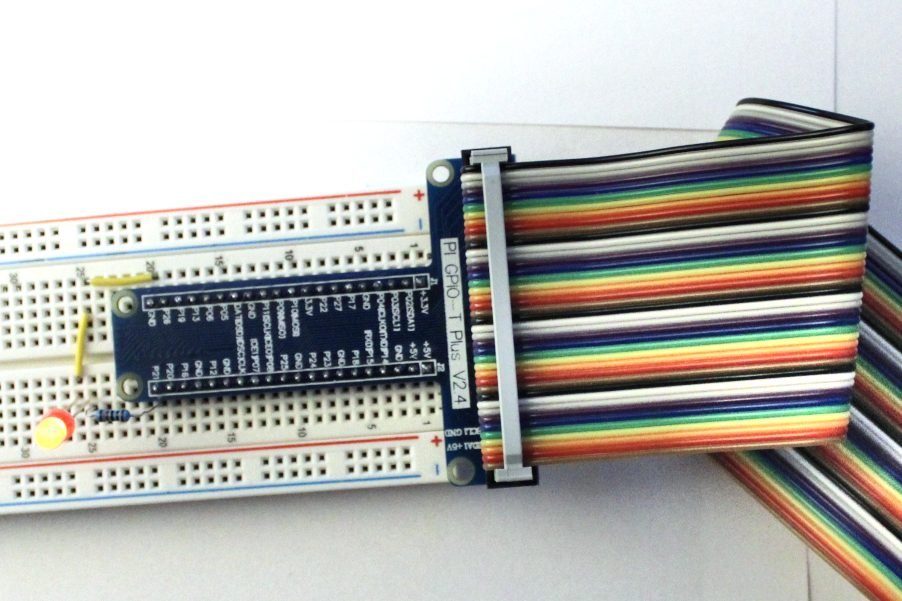
\includegraphics[width=\textwidth]{img/led_direkt_foto}
    \end{columns}
\end{frame}
}

%%% Folie
{
\scriptsize

\begin{frame}{Mittlere Lasten über Transistor schalten}
    \Justified{
        Aus Softwaresicht macht es keinen Unterschied, ob über einen GPIO-Pin eine simple
        LED, einer Motor oder irgend eine andere Last geschaltet wird. Aus Hardwaresicht
        gilt lediglich zu beachten, dass der Raspberry Pi nur \textbf{sehr kleine Ströme}
        abgeben kann, die somit am ehesten als Steuerströme beispielsweise zum Schalten eines
        Transistors oder eines Relais genutzt werden können.
        \smallskip

        Der hier gezeigte ,,NPN-Transistor'' funktioniert im einfachsten Fall wie ein
        \textbf{stromgesteuerter Schalter}. \textcolor{RoyalPurple}{Ein kleiner Strom
        an der Basis steuert, in wiefern ein viel größerer am Collector anliegender Strom
        durchgelassen wird. Die Summe beider Ströme (in Ampére) fließt durch den Emitter
        nach Ground.}
        \smallskip

        Die Spannung zwischen Basis und Emitter muss meist mindestens 0,7V betragen,
        damit der Transistor schalten kann. Die Stärke des hierfür benötigten
        Steuer- bzw. Basisstroms kann mit der durchzuschaltenden Stromstärke, dem
        $\beta$-Faktor des Transistors, (auch \texttt{hfe} abgekürzt) und dem Ohmschen
        Gesetz leicht berechnet werden:
        \bigskip

        \hfill $I_b = I_c / \beta$ \hfill
        \hfill \textit{Benötigter Basisstrom = Zu schaltender Strom / $\beta$} \hfill
        \smallskip
    }

    \bigskip

    \begin{columns}[T]
        \column{0.5\textwidth}
        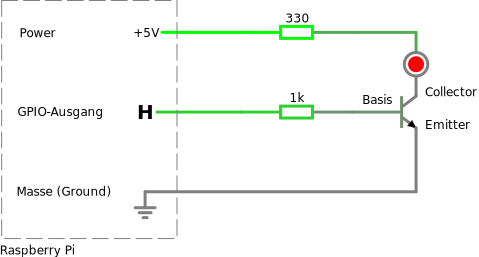
\includegraphics[width=\textwidth]{img/led_transistor_circuitjs}
        \smallskip

        \CircuitJS{https://www.falstad.com/circuit/circuitjs.html?ctz=CQAgjCAMB0l3BWcMBMcUHYMGZIA4UA2ATmIxAUgoqoQFMBaMMAKABkRiAWLkLsQiDxc8fAVHAgAZgEMANgGc6IbNGxQWAcyEi+xQcNEIwKCZBYB3cCapd9O0XcHmASpx4rsB3di9m+tP4wCCwATu68-IJgkAiCURIxcCwALshxYtE2mYlQ0IRgxGCU3Hh4xJAouLwwhIR2cAII2GQIzbxJIAAmdLIArnIpltZofNimzKNOGuHcvL7RsYILEr7mVjEZK5NUK+YARkJ4u5C8GKcUXOrmAB4g56ZtxPdYFISmHaYuMgoADvt0UKhACeAB0FAAFACWLDuGBQpmw-HuCFESMi4FMEIA9hZAbD7lNRsd4lU+JiQABxCEASQA8gwAIJ9BSaGQAO00BIwhRoVDwYHUlHUnxAAFkfkpwQAKSmhbF9dldACULAEE2y22yXDgIFMPX6gwYcjoXUkVAtsFYdxidQCohiZDEEFFACEflCFATJs8dVRmAQAiKKQBhbFyE0AYxS2NC3pMvt81hwY3iFIAogBbKEpFL4oA}
        \LinkButton{https://www.electronics-tutorials.ws/de/transistoren/der-npn-transistoren.html}{NPN-Transistoren im Detail}

        \column{0.42\textwidth}
        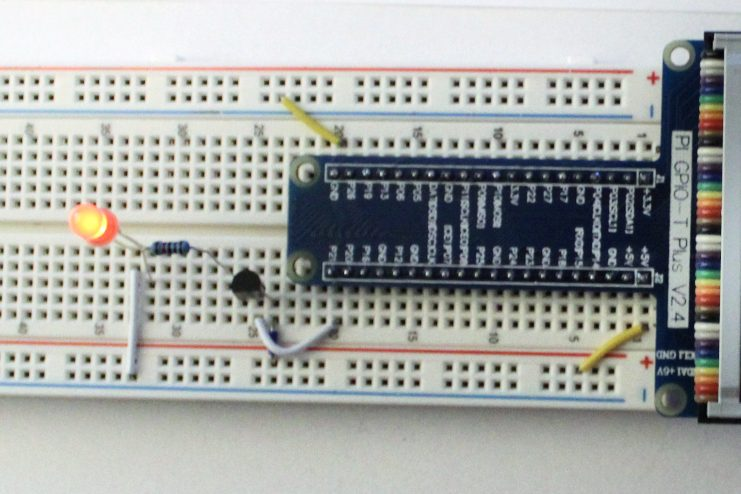
\includegraphics[width=\textwidth]{img/led_transistor_foto}
    \end{columns}
\end{frame}
}

%%% Folie
{
\scriptsize

\begin{frame}{Große Lasten über Relais schalten}
    \Justified{
        Große Lasten sollten aus Sicherheitsgründen eher mechanisch geschaltet werden.
        Der Hardwareaufbau gliedert sich dann ein einen \textbf{Steuerstromkreis} und
        einen \textbf{Arbeitsstromkreis}, die komplett \textbf{galvanisch entkoppelt}
        sind und deshalb jeweils eigene Stromquellen besitzen.
        Ein \textbf{Relais} dient als ferngesteuerter Schalter, der den Arbeitsstromkreis
        unterbrechen und schließen kann. Im Inneren besteht es aus einem durch den
        Steuerstromkreis gespeisten Elektromagneten und einem magnetischen Kippschalter.
        Beim Umschalten entsteht das charakteristische Klickgeräusch.
    }

    \medskip

    \begin{columns}
        \column{0.6\textwidth}
        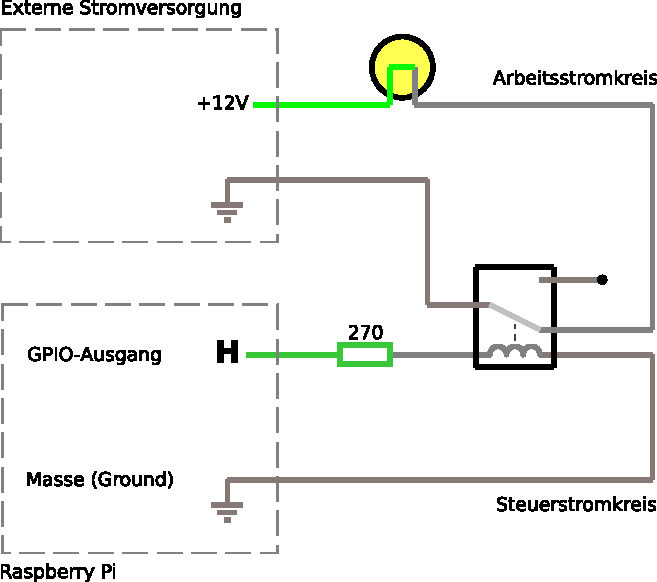
\includegraphics[width=.9\textwidth]{img/led_relais_circuitjs}
        \smallskip

        \CircuitJS{https://www.falstad.com/circuit/circuitjs.html?ctz=CQAgjCAMB0l3BWcMBMcUHYMGZIA4UA2ATmIxAUgoqoQFMBaMMAKABkQ9jCQAWMHnl54+AqOBAAzAIYAbAM50Q2aNigsA5p2F9u2kQjApxkFgCdOe-jzI9r4zKYBGnPFWxCQGSLwq81pgAeXpDGCAjEXlgUhMa+RiAAStLyAA5OdGZmAJ4AOvIACgCWLMEYaHwVbnYoavHGAOIFAJIA8gwAggCu8hrSAHYapV5gkZRUeGBqlHXgxgCyKYr5ABQNZgD2Xf0AJgCULGAYIrbKnmD4Ih6+PBCoULDM2BjE2BfYvMKYvITkMJBIC7wOAPSAQCr-HyggHgFgAd3ARio9mYFV4elMCNRyL0QhE6J4QWQFUMtyMYVGfDmIAAygAXOhdTLyOmbAC2AGszHQivJDpNLDwUAhbqFfMLCeBiCheLAhIZuJQpngeJRqf9fBr4YiKhKdciQZjkHh8SDsXxDdrzSjLqJCcMLmARDK1Ki1DK7NSOmYMkU6fIWeyuTy+Vo8cooeHsBD1Aio1DTrhNdrEwmMDxrupEoKQHrw3qqAb1SZoAgrWLcyL9ZX7S4TVQ0CJvGoPsmypBXcQRHgEOQ0BB6iAAKKBBlmfp0fL09kAN2ZGzMGm2QyAA}

        \column{0.4\textwidth}
        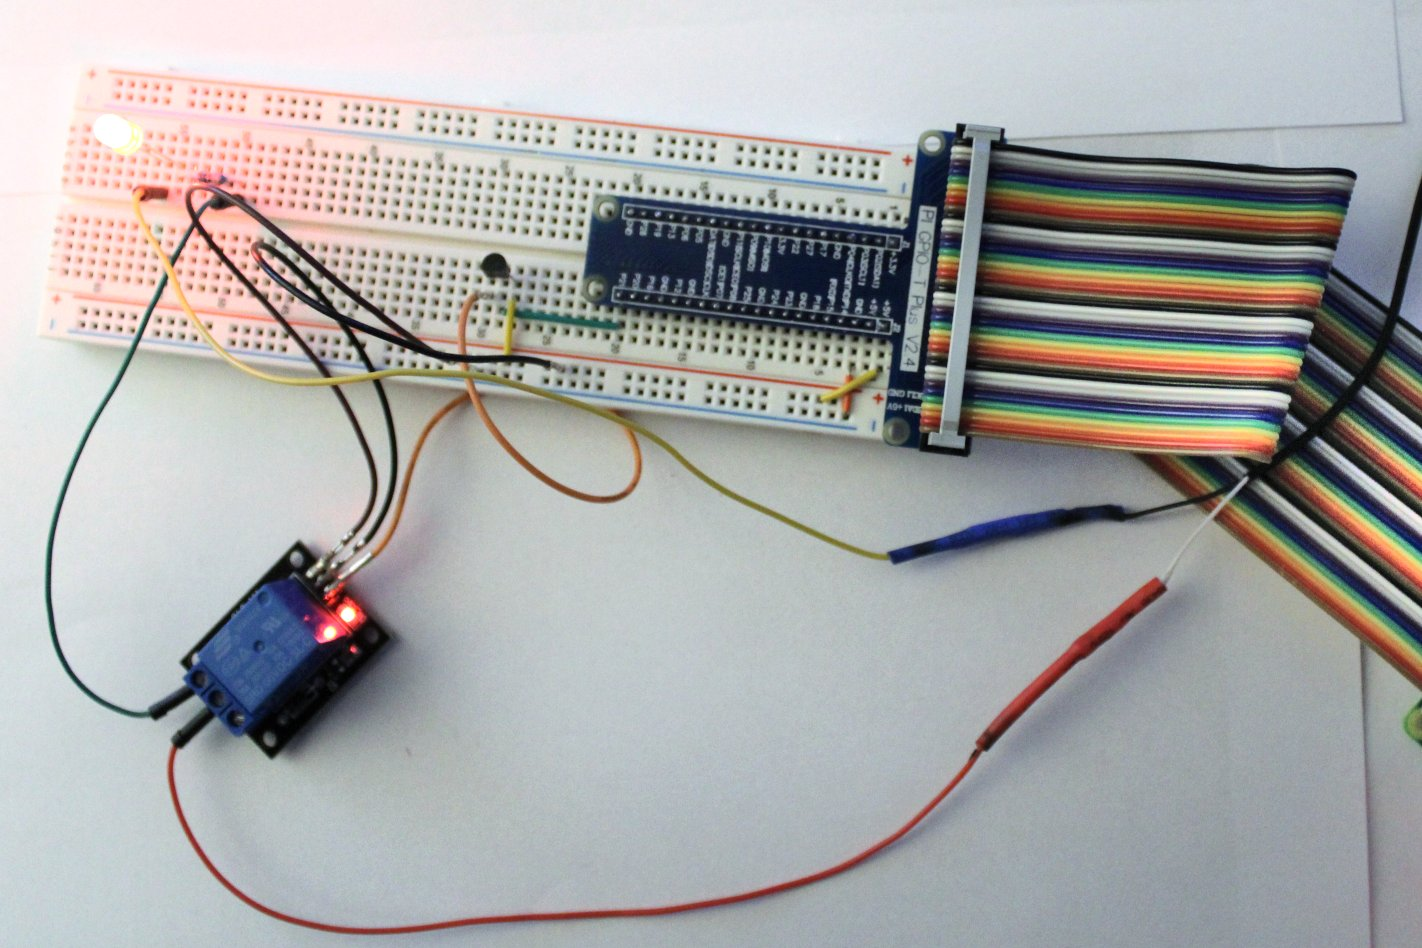
\includegraphics[width=\textwidth]{img/led_relais_foto}
    \end{columns}
\end{frame}
}

%%% Folie
{
\scriptsize

\begin{frame}{Inkompatible Logikpegel anpassen} % mit Transistor
    \Justified{
        Ein ähnliches Problem wie beim Schalten starker Ströme ergibt sich, wenn digitale
        Bausteine mit inkompatiblem Logikleven mit dem Raspberry Pi verbunden werden sollen.
        Anstelle der Stromstärke muss hier jedoch die \textbf{Spannung} angepasst werden.
        \smallskip

        Denn nicht alle digitalen Geräte arbeiten mit einem Logikpegel von 3,3\,V. Insbesondere
        ältere Geräte nutzen 5\,V, während heutzutage auch 1,8\,V oder kleinere Spannungen
        üblich sind. Passt der Logiklevel eines Bauteils nicht zum Raspberry Pi, kann es
        daher entweder zu Beschädigungen oder einem unzuverlässigen Datenaustausch kommen.
        Auf folgende Weise kann der Potentialunterschied dann ausgeglichen werden:
    }

    \begin{itemize}
        \item Mit zwei Widerständen als Spannungsteiler
        \item Mit in Reihe geschalteten Dioden zum Absenken einer Spannung
        \item Mit einem Transistor als stromgesteuerter Schalter
        \item Mit einem integrierten Baustein wie dem 74HC04050
    \end{itemize}
    \medskip

    \begin{columns}
        \column{.5\textwidth}
        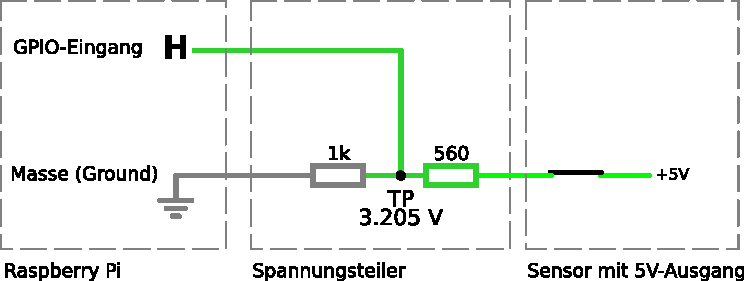
\includegraphics[width=\textwidth]{img/logiklevel_spannungsteiler}

        \column{.5\textwidth}
        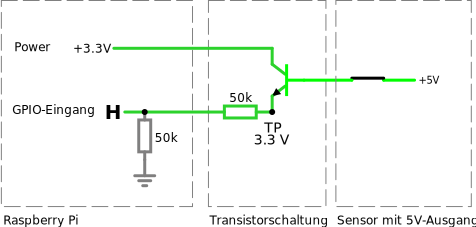
\includegraphics[width=\textwidth]{img/logiklevel_transistor}
    \end{columns}
    \medskip

    \begin{columns}
        \column{.5\textwidth}
        \LinkButton{%
            https://www.falstad.com/circuit/circuitjs.html?ctz=CQAgjCAMB0l3BWcMBMcUHYMGZIA4UA2ATmIxAUgoqoQFMBaMMAKACURSURs1kAWKryoiQg6qJgIWAZ06EhfLjz6iAZgEMANjLosATpxR4VVPIX6moFBQZDnLwkBjyPVyOCwDu9iyBTiDlaQLACyzq7+4hh8AaLY3r6WcRHJ4iEA5s58TjFC2ITWIT4ublR5wSwARs4I3GgmCiYF5CE1GIQmDZzYjoSticQKVsTGlTXE-Mn4yHhC-VAsAB4ghGBCeEidSNh4JpZg3GwaMgAOVXT6+gCeADoyAAoAlsvOJDybvoW7++DcAMqnDQAO2BAFdgRkZAAXOhPLSXV6THafdaRH5iP4gf50YEyAD2+nuAFsntD7ggAGoMACCYJkGRBGVea0KAW4JC6-CQB24AHEHgBJADyDAAok9IUyWWA3NhnDNeIVeSBQiddPcABR8-T4iEAEwAlCwCiYgk5zQUiiwgA
        }{
            Spannungsteiler online ausprobieren
        }

        \column{.5\textwidth}
        \hfill
        \LinkButton{%
            https://www.falstad.com/circuit/circuitjs.html?ctz=CQAgjCAMB0l3BWcMBMcUHYMGZIA4UA2ATmIxAUgoqoQFMBaMMAKACURSUQU89kALFV78qVIdTFRoCFgGdOhYX07FuIqJoBmAQwA2cuiwBGIPHB74QS-gLBJIJs2EKX+xbAJB2HLAO6Kyu5g6iqOpsQCXmj8YPji9lAsAB7Wcd7Y2NZ4SALYrl4hIGw6cgAOxnQATlUAngA6cgAKAJYpzuR5WR5ZeQXg3AAqVToAdnItcgAuAPZVcgDGABb6UwCuowDm7ZG5mch4Xn3eAyAAynTjc40Ati1TjQgAagwAgmtym2PbHHzCCK4MJBogDNOIqNhoFkpDBZKlCCgICgEMRrAhyERuIVuE0Zn5qiwppwiho-jwwuBwNAgfBaXTINwwNASGQBERPCQUAICOQ4lQACZ0XRrPRTfxmcw8DDcMnI1yOKrOVzYNASiGq2i08VklVUHXApIAWRAGAQ3F1JtVFuEMnahDAqJV3CBEBVuVOAHEmgBJADyDAAoi0tt8WJsTWaQPl+KbzYcwSxFbGo6rk9HNJR4OK06q8C4U2IWOmdbnJZl5UkgA
        }{
            Transistorschaltung online ausprobieren
        }
    \end{columns}
\end{frame}
}

%%% Folie
{
\scriptsize

\begin{frame}{Gemittelte Leistung durch Pulsweitenmodulation regulieren}
    \parbox{\linewidth}{
        Die zur Verfügung stehende Stromstärke kann nicht nur durch einen Vorwiderstand reduziert werden.
        Je nach Bauteil kann (oder muss) sie durch \textbf{Pulsweitenmodulation}, was einem schnellen
        Ein- und Ausschalten entspricht, im zeitlichen Mittel reduziert werden. Die zwei wesentlichen
        Parameter sind die \textbf{Frequenz} und der \textbf{Tastgrad} (Duty Cycle):
    }

    \begin{center}
        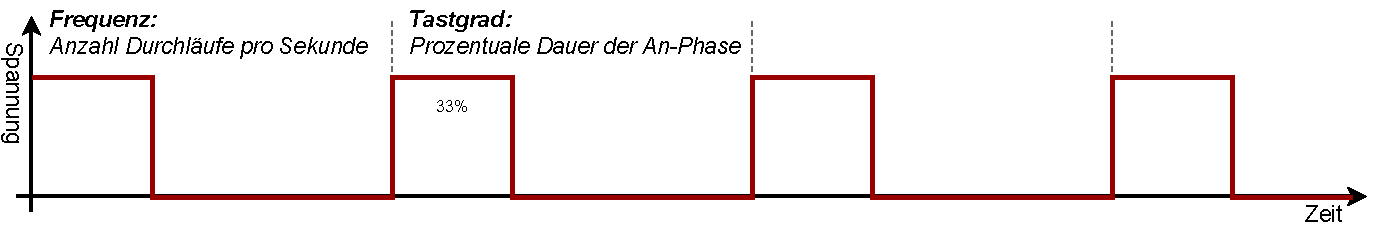
\includegraphics[width=.8\textwidth]{img/pwm} \\
        \bigskip

        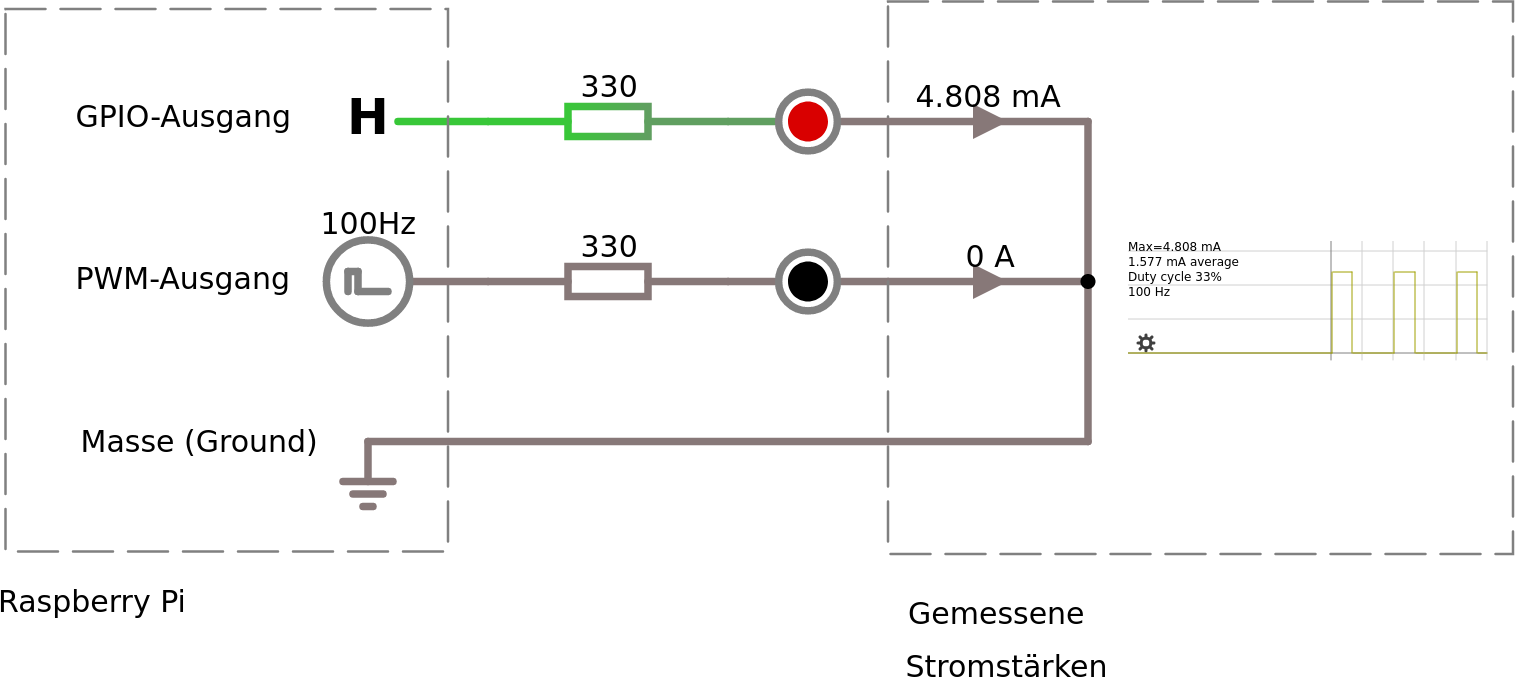
\includegraphics[width=.75\textwidth]{img/led_pwm_circuitjs}
    \end{center}

    \hfill
    \CircuitJS{https://www.falstad.com/circuit/circuitjs.html?ctz=CQAgjCAMB0l3BWcMBMcUHYMGZIA4UA2ATmIxAUgoqoQFMBaMMAKAHMRCUAWCsFTjwoo8UKCwBOnDAO7dRGQqLmiq2XCzBcQi5fJB5ss-QIAmdAGYBDAK4AbAC4M7dU+DFUYkVgBlpA7DxeLl5A3ioIazsAZzoQbGhscSlCGXignSV08PiNbAwqQwCM4n5s908WfMKjEBUQUuNRCEqAdwaysI6m8XbGuv1+hDLIFj6y4YEQvgFRgCNOBEJc4jqMVYQl8QAPNeWEPFphikM68AEAJStogAc5ugkJAE8AHWiABQBLFl3KDa1OJAksNVrwygBZa6xN4ACgA4hIAPY2AB2pgAlD8aORAvtiElAqDziA4e8AJIAeQYAEEbNE2FYUWwsZRyNxjghiLIELwwQJ3gB1cE0ukMpksBZFXLLMD4ASbcijXZBWh4JClVXKYlwugAWzo0ViKLoWMMq0IkGWpXNkCJZQAyg4kbrog4ACcSADWdBRmm0unKUq6ZkstkczlcFQ8sFYF38A1E03qvCQsrUiQ8UES2BY3CBDREdVqsrS8k8nAA+kYK5AK1p1uya7B4IoUPjiOzsPwEE24Fwe7WUBXCFWWEA}
\end{frame}
}

%%% Folie
{
\small
\setlength{\leftmargini}{1.2em}

\begin{frame}{Pulsweitenmodulation am Beispiel eines Servomotors}
    \begin{columns}[onlytextwidth]
        \column{.49\textwidth}
        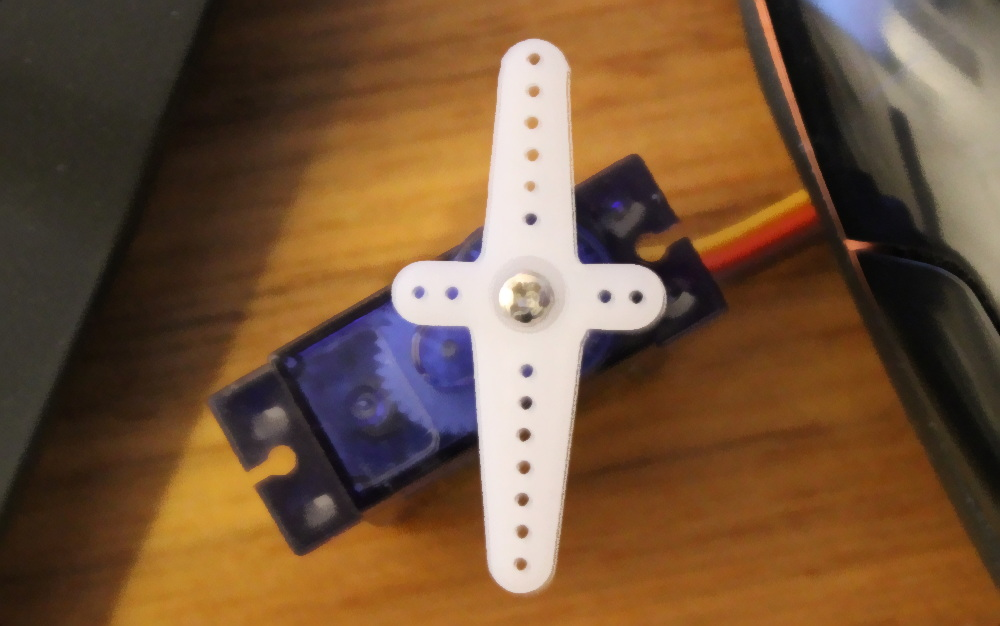
\includegraphics[width=\textwidth]{img/servomotor-foto1}

        \column{.49\textwidth}
        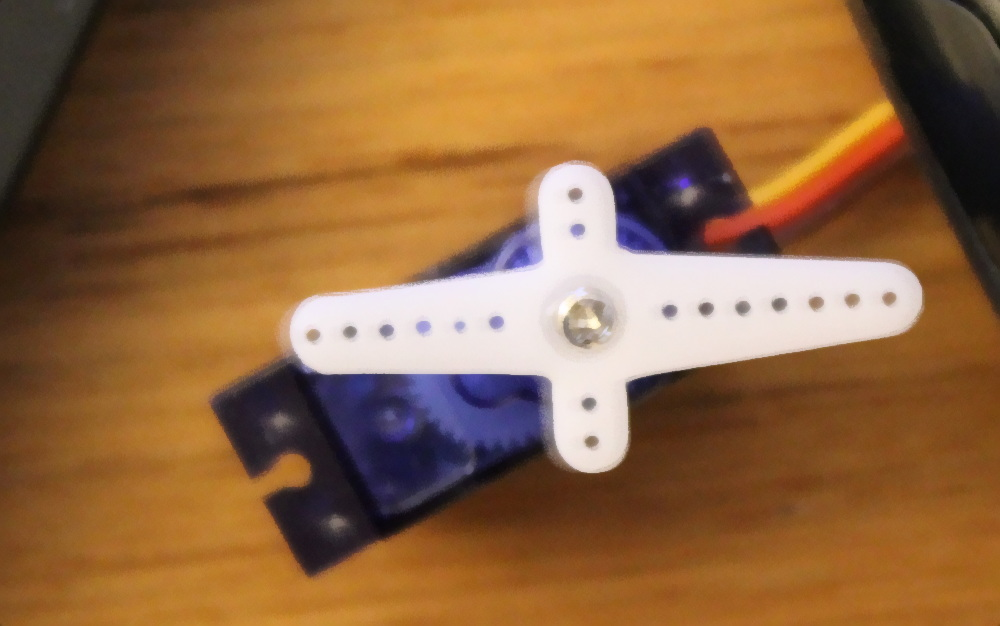
\includegraphics[width=\textwidth]{img/servomotor-foto2}
    \end{columns}

    \bigskip
    Steuerung eines Servomotors mit Pulsweitenmodulation. Die Länge des Lastzyklus
    bestimmt die Position:

    {
        \footnotesize
        \smallskip
        \begin{itemize}
            \item \textbf{Ganz links:} 1\,ms Puls bei 50\,Hz Frequenz
            \item \textbf{Ganz rechts:} 2\,ms Puls bei 50\,Hz Frequenz
            \item \textbf{Andere:} Jeder Wert dazwischen
        \end{itemize}
    }

    \begin{columns}[onlytextwidth]
        \column[T]{.3\textwidth}
        \begin{block}{Hardwareskizze}
            \smallskip
            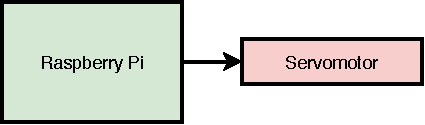
\includegraphics[width=\textwidth]{img/servomotor-skizze}
        \end{block}

        \column[T]{.59\textwidth}
        \begin{block}{Schaltplan}
            \smallskip
            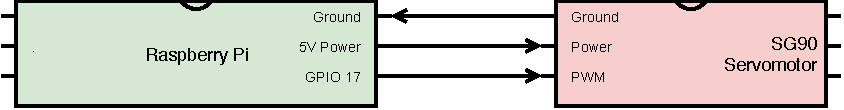
\includegraphics[width=\textwidth]{img/servomotor-schaltplan}
        \end{block}
    \end{columns}
\end{frame}
}

%%% Folie
{
\scriptsize

\begin{frame}{Digitaleingang mit Active-High-Logik (z.B. Taster)}
    \Justified{
        Viele Sensoren stellen lediglich einen \textbf{Kontakt zwischen zwei Pins} her, wenn ein bestimmtes
        Ereignis eintritt, zum Beispiel wenn ein Schalter gedrückt, eine Berührung mit einem Hindernis
        oder ein Feuer erkannt wird. Indem man einen Pin des Sensors mit einer 3,3\,V Versorgungsspannung
        und den anderen Pin mit einem GPIO-Eingang verbindet, lässt sich eine sog. \textbf{Active-High-Logik}
        realisieren. Dies bedeutet, dass der GPIO-Eingang durch den Sensor mit 3,3\,V gespeist wird,
        wenn das Ereignis eintritt, was vom Raspberry Pi als logische Eins interpretiert wird.
        \smallskip

        Jedoch sollte in diesem Fall immer der \textbf{interne Pull-Down-Widerstand} des Raspberry Pi
        aktiviert werden, um den Eingang auf Masse zu ziehen, wenn kein Signal anliegt. Andernfalls
        führen \textbf{parasitäre Induktionen} zu zufälligen Phantomwerten und Fehlmessungen.
        \medskip
    }

    \begin{columns}
        \column{0.6\textwidth}
        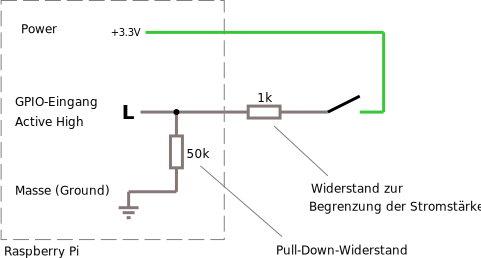
\includegraphics[width=\textwidth]{img/button_pulldown_circuitjs}
        \bigskip

        \CircuitJS{https://www.falstad.com/circuit/circuitjs.html?ctz=CQAgjCAMB0l3BWcMBMcUHYMGZIA4UA2ATmIxAUgoqoQFMBaMMAKAFkQ9sUQAWPKjkJ8BUECmgIWADxCEUPXhl4gMkFUvIqwPAOIAFAJIB5BgFEAlgDsA5gENbLAM4hiOkVVKLRVCADM7ABsnOhYAJU5uPjhVbGFeGKoqBJBsaGwxJMkWG1jhBEJBOIoMYSSWAHc8ikLVPBUC8oAnOo1RDHqapJp4GTkFPmIVEmSyPnAeAEEAYwAXCwA3OgAdJwAJCxsACz75HgKMjDB8wniJkDY7JxDVgApdJoB7AFcrABMASkrXYm9PX+i5SqXkBkUUiRYLS4f1c7n43TAvVkeE68gyiLASHkZ3c+megUCDAAIo8KlYGAB1CxvOhNJyzBxvPpucgIDDEZB4DkIAjjdwAIToNiadCsAC9XjZVjSmqsAMqzJ4AW3pABOmgBrUKyNzcwgQDG0Qgac5UmX0xmrCVNFi8FAZYjFBC8FQoxRDKC2+2cYhUQpIAR4CjYFSQFgAIzBqUIQcKsfwntk8iDCQgpw06j5PH0pNpu2Y-WGeGE8i05zCVwADuHaU0AJ6rfQWFhAA}

        \column{0.4\textwidth}
        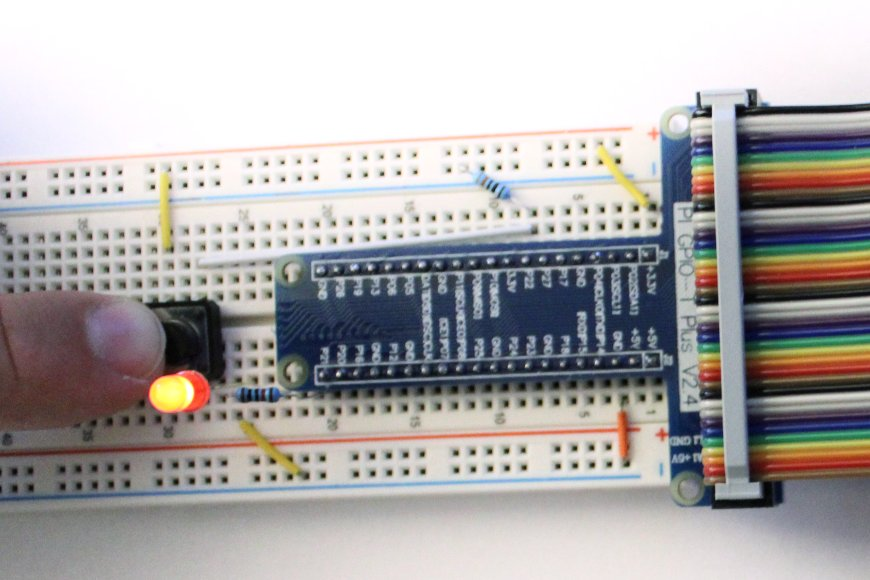
\includegraphics[width=\textwidth]{img/button_pulldown_foto}
    \end{columns}
\end{frame}
}

%%% Folie
{
\scriptsize

\begin{frame}{Digitaleingang mit Active-Low-Logik (z.B. Lichtschranke)}
    \Justified{
        Einige Sensoren \textbf{unterbrechen einen Kontakt}, wenn die festzustellende Bedingung eintritt.
        Dies trifft zum Beispiel auf Lichtschranken zu, die an ihrem Ausgang so lange einen Strom liefern,
        bis sie unterbrochen werden. Am einfachsten lassen sich solche Sensoren wie hier gezeigt mit einer
        \textbf{Active-Low-Logik} verbinden.
        Indem der interne Pull-Up-Widerstand des Raspberry Pi aktiviert wird, wird der GPIO-Eingang bei
        einer Unterbrechung des Eingangssignals auf eine logische Eins hochgezogen. Die meiste Zeit kann
        der Strom jedoch über den Sensor nach Masse abfließen, so dass der Raspberry Pi stattdessen eine
        logische Null sieht.
    }

    \bigskip

    \begin{columns}
        \column{0.6\textwidth}
        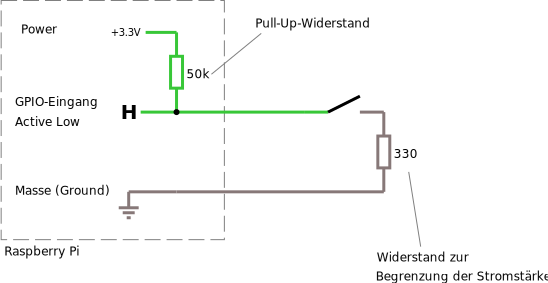
\includegraphics[width=\textwidth]{img/button_pullup_circuitjs}
        \bigskip

        \CircuitJS{https://www.falstad.com/circuit/circuitjs.html?ctz=CQAgjCAMB0l3BWcMBMcUHYMGZIA4UA2ATmIxAUgoqoQFMBaMMAKAFkQM8AWEbvKjkJ8BUECmgIWADxCEUKPhl4ZIvblj7hFAcQAKASQDyDAKIBLAHYBzAIY2WAZxDEwi-lVLvRVCADNbABtHOhYAJU4ePjhObGFuGKoqBJBsaGwxJMkWa1jhBEJBOIoMYSSWAHc8ikLI3gLygCc66MEojzFKeBk5BT5iXkI8eLItNxAAQQBjABdzADc6AB1HABkAewqe+UUCjIwwfMJ47RA2W0cQlYAKHUb1gFdLABMASkqXYl3arnrayB6wwy2GISDI5BBeDGij0D0CgQYAFUAA4MADq5medEajhm9meLG4KAyw2I0QgeDAZO4RKgLAARiA8NhFHEoYV2fg6bJ5FCEhBjuo1NCQHpNtjtsxeoNhr1yLxxmELsj6djGgBPFZ6cwfVzeNrqHwsZpeESeL41JKpXA9Yh4JCEXDIUpybAZBWKDFYnF4l4rABeD0atqihG4ZOYBTkCHcpwAQnRrI06JZAzYVt6VgBlGb3AC2uIAJ40ANahIkZMCQFBkwhgJBVsDkBApAFAA}

        \column{0.4\textwidth}
        \includegraphics[width=\textwidth]{img/button_pullup_foto}
    \end{columns}
\end{frame}
}

%-------------------------------------------------------------------------------
\section{Serielle Kommunikation}
%-------------------------------------------------------------------------------

%%% Folie
\begin{frame}{Einsatzgebiete serieller Schnittstellen}
    \begin{columns}
        \column{\dimexpr\paperwidth-28pt}
        \begin{itemize}
            \item Kommunikation zwischen den Komponenten eines eingebetteten Systems
            \item Datenaustausch zwischen getrennten Subsystemen und anderen Computern
            \item Anbindung von Sensoren und Aktoren an Eingebettete/IoT-Devices
        \end{itemize}
    \end{columns}

    \bigskip
    \bigskip
    \bigskip

    \begin{columns}
        \column{.33\textwidth}
        \includegraphics[width=\textwidth]{img/seriell_einsatz1}

        \column{.33\textwidth}
        \includegraphics[width=\textwidth]{img/seriell_einsatz2}

        \column{.33\textwidth}
        \includegraphics[width=\textwidth]{img/seriell_einsatz3}
    \end{columns}
\end{frame}

%%% Folie
{
\footnotesize

\begin{frame}{Funktionsweise der seriellen Datenübertragung}
    \begin{columns}
        \column{\dimexpr\paperwidth-28pt}
        \parbox{\textwidth}{
            Serielle Schnittstellen übertragen digitale Daten durch schnelles Umschalten
            der Logikpegel einer einzigen Datenleitung. Die Schnittstellenart gibt dabei
            vor, wie die Logikpegel in elektrische Signale umgewandelt werden, welche
            Geschwindigkeiten zulässig sind und wie sich Sender und Empfänger synchronisieren.

            \medskip
            \begin{itemize}
                \item \textbf{Synchron:}
                Synchronisation über ein zusätzliches Taktsignal (Serial Clock)

                \item \textbf{Asynchron:}
                Synchronisation über Synchronisationsbits im Datensignal
            \end{itemize}
        }

        \medskip
        \includegraphics[width=\textwidth]{img/seriell_arten}
    \end{columns}
\end{frame}
}

%%% Folie
{
\small

\begin{frame}{Verbreitete serielle Schnittstellen}
    \begin{columns}
        \column[T]{.5\textwidth}
        \textbf{Universal Asynchronous Receiver Transmitter (UART)} \\
        \smallskip
        \includegraphics[width=\textwidth]{img/seriell_uart_schaltplan}

        \column[T]{.5\textwidth}
        \textbf{Serial Peripheriel Interface (SPI)} \\
        \smallskip
        \includegraphics[width=0.8\textwidth]{img/seriell_spi_schaltplan}
    \end{columns}

    \medskip

    \textbf{Inter-Integrated Circuit (I²C)} \\
    \smallskip
    \includegraphics[width=\textwidth]{img/seriell_i2c_schaltplan}
\end{frame}
}

%%% Folie
{
\scriptsize

\begin{frame}{Beispiel: DHT11-Umweltsensor}
    \parbox{\linewidth}{
        Der DHT11-Sensor misst alle zwei Sekunden Temperatur und relative Luftfeuchtigkeit.
        Die Werte werden über das serielle 1-wire-Protokoll als \textbf{digitaler Datenstrom} übertragen.
        1-wire ist dabei ein serielles Protokoll, das mit nur einer Datenleitung auskommt, da es
        nur einen Sender und einen Empfänger gibt und die \textbf{Synchronisation über das Datensignal}
        erfolgen kann.
    }
    \bigskip

    \begin{columns}
        \column[b]{0.7\textwidth}
        \includegraphics[width=\textwidth]{img/dht11_schaltplan}

        \column[b]{0.3\textwidth}
        \includegraphics[width=\textwidth]{img/dht11_foto1}
        \includegraphics[width=\textwidth]{img/dht11_foto2}
    \end{columns}
\end{frame}
}

%%% Folie
{

\scriptsize

\begin{frame}{Beispiel: A/D-Konverter}
    \begin{columns}[onlytextwidth]
        \column{.49\textwidth}
        \includegraphics[width=\textwidth]{img/lautstaerke-foto1}

        \column{.49\textwidth}
        \includegraphics[width=\textwidth]{img/lautstaerke-foto2}
    \end{columns}
    \medskip

    \Justified{
        Der Raspberry Pi kann Analogsignale weder erzeugen noch messen. Mit Hilfe eines
        externen \textbf{Analog/Digitalwandlers} (A/D-Konverters) lassen sich analoge
        Spannungsverläufe jedoch leicht messen und als \textbf{serieller Datenstrom}
        übertragen. Zur Erzeugung analoger Signale kann entweder ein D/A-Wandler als
        externer Baustein genutzt oder mit einer Handvoll Widerständen nachgebaut
        werden (sog. \textbf{R2R-Leiter}).
    }
    \medskip

    \includegraphics[width=\textwidth]{img/lautstaerke-schaltplan}
\end{frame}
}

%%% Folie
{
\tiny
\setlength{\fboxsep}{0pt}

\begin{frame}{Exkurs: Analogsignale erzeugen ohne D/A-Wandler}
    \Justified{
        In der Regel würde man zur Erzeugung eines Analogsignals wie im Vorherigen Beispiel
        über die serielle Schnittstelle einen D/A-Wandler anbinden. Wenn man aber noch ein
        paar GPIO-Ausgänge frei hat und das Ausgangssignal nicht sehr präzise sein muss,
        kann man einen einfachen D/A-Wandler mit ein paar Widerständen als sog. \textbf{R2R-Leiter}
        diskret aufbauen.
    }
    \smallskip

    \begin{center}
        \fbox{\includegraphics[width=.9\textwidth]{img/r2r-leiter}}
    \end{center}
    \smallskip

    \LinkButton{%
        https://www.falstad.com/circuit/circuitjs.html?ctz=CQAgjCAMB0l3BWcMBMcUHYMGZIA4UA2ATmIxAUgoqoQFMBaMMAKABkRiAWLkLsQiDwC+IqlQBmAQwA2AZzohs0bFHacefYoOGCu2qIenzFy1ZHXdeCDDpE3B4kMYVKVajlZCEEdwT8cjWVczNQAnDV5+QTBIX1FAlDQLCK99GLi9AyokuBZUzQdkeKKc5PzI73jY+IDDXJTi-2rMiltDZjyImsEinq1Azsb+9KaEjtiLAHMhEQw0WcEcQIsAd0WQeaowFC48TYWLAAdwXf26nb2D7cM1sYuzqscKkZF+7GxE8pndJU+N7AIFC3FjrX4fDLxCFqABG4DAQO8XG22AWtn2FjhXlwvGYzE2hAxLDheDwVBx3mwxAJRIAHkjVBg8IywPsmXpTiAAEpSORHGF0MJhACeAB05AAFACWLHpxAQvHZyBQbLw1NxwIAIgB6ACCDAA6lIAHYAExkgtl8IQSCZGpQtrw5A1IAA4nQALZ0OQKY10K3MBVCSDAnYYCBkpAu3UAVzkUxNUx9RxNxpjxqmVsIhFU2GRmxsSi4qhdAFleQpxQAKV1hAD26dNAEos4RgfNFfF5s7OeWfXRq7WG2aW-Ts1EwNSmVGknxOa6JQBJADyDFj8cTAC5xQAhKUAF3FFjHOa0U7w1hDc52bqXq-XCYz27ke8PcmP3lPNlV1mE1+BC4rmucaPlMz6vkeraqD4568NmwIuoB94gVuu4HpBdbgNBvBUMixAYtAbZIDAEDbCwQA
    }{R2R-Leiter online ausprobieren}
\end{frame}
}

%-------------------------------------------------------------------------------
\section{Programmierung in Python}
%-------------------------------------------------------------------------------
%%% Folie
\begin{frame}{Quellcodes und Dokumentationen}
    \LinkButton{https://github.com/DennisSchulmeister/dhbwka-mt-iot-quellcodes}{Quellcodes auf GitHub}
    \LinkButton{https://sourceforge.net/p/raspberry-gpio-python/wiki/Examples/}{Dokumentation zu RPi.GPIO}
    \LinkButton{https://gpiozero.readthedocs.io/}{Dokumentation zu gpiozero}
    \LinkButton{https://docs.circuitpython.org/projects/bundle/en/latest/drivers.html}{CircuitPython Libraries}

    \smallskip
    \setlength{\fboxsep}{0em}
    \fbox{\includegraphics[width=\textwidth]{img/github}}
\end{frame}

%%% Folie
{
\footnotesize

\begin{frame}{Hardware- vs. Softwaresicht}
    \Justified{
        Grundsätzlich spiegelt sich der physische Hardwareaufbau nur sehr rudimentär in
        der Software wieder, da aus Softwaresicht meist nur digitale Ausgänge geschaltet
        oder Eingänge überwacht werden. Jedoch kann die Software auf unterschiedlichen
        Abstraktionsebene programmiert werden, wodurch es möglich wird, die Elemente der
        realen Welt auf Elemente der virtuellen Welt abzubilden und somit die Wirkungsweise
        des Quellcodes besser zu dokumentieren.
    }
    \medskip

    %%%% TODO: Bilder
    \begin{columns}[b,onlytextwidth]
        \column{.48\textwidth}
        \textbf{Hardwarenahe Programmierung¹}

        \column{.48\textwidth}
        \textbf{Imperative Programmierung}
    \end{columns}
    \medskip

    \begin{columns}[b,onlytextwidth]
        \column{.48\textwidth}
        \textbf{Deklarative Programmierung}

        \column{.48\textwidth}
        \textbf{Objekt-orientierte Programmierung}
    \end{columns}
    \vfill

    \Justified{
        \tiny
        ¹ Hardwarenahe Programmierung bezieht sich hier auf die Computer-Hardware.
    }
\end{frame}
}

%%% Folie
\begin{frame}[fragile]{Beispiel: LED-Ansteuern (imperativ)}
    \begin{lstlisting}[language=Python, gobble=8]
        import RPi.GPIO as GPIO, time

        GPIO_LED = 21
        DELAY_S = 0.5

        if __name__ == "__main__":
            try:
                # GPIO-Pin initialisieren
                GPIO.setmode(GPIO.BCM)
                GPIO.setup(GPIO_LED, GPIO.OUT)

                # LED alle halbe Sekunde ein bzw. ausschalten
                led_status = False

                while True:
                    led_status = not led_status
                    GPIO.output(GPIO_LED, led_status)

                    print("LED ist an" if led_status else "LED ist aus")

                    time.sleep(DELAY_S)
            except KeyboardInterrupt:
                pass

            GPIO.cleanup()
    \end{lstlisting}
\end{frame}

%%% Folie
\begin{frame}[allowframebreaks,fragile]{Beispiel: LED-Ansteuern (deklarativ)}
    \begin{center}
        \includegraphics[width=.33\textwidth]{img/gpiozero-led-button}
    \end{center}
    \bigskip

    \begin{lstlisting}[language=Python, gobble=8]
        from gpiozero import LED, Button
        from signal import pause

        led = LED(17)
        button = Button(2)

        # LED wird durch den Button gesteuert
        led.source = button

        pause()
    \end{lstlisting}

    \framebreak

    \begin{center}
        \includegraphics[width=.8\textwidth]{img/gpiozero-garden-light}
    \end{center}
    \bigskip

    \begin{lstlisting}[language=Python, gobble=8]
        from gpiozero import LED, MotionSensor, LightSensor
        from gpiozero.tools import booleanized, all_values
        from signal import pause

        garden = LED(2)
        motion = MotionSensor(4)
        light = LightSensor(5)

        garden.source = all_values(booleanized(light, 0, 0.1), motion)

        pause()
    \end{lstlisting}
\end{frame}

%%% Folie
\begin{frame}[fragile]{Beispiel: Pulsweitenmodulation (imperativ)}
    \begin{lstlisting}[language=Python, gobble=8]
        import RPi.GPIO as GPIO, time

        GPIO_LED   = 12
        FREQUENCY  = 100    # 100 Hz
        DUTY_CYCLE = 50     # 50%

        if __name__ == "__main__":
            try:
                # GPIO-Pin initialisieren
                GPIO.setmode(GPIO.BCM)
                GPIO.setup(GPIO_LED, GPIO.OUT)

                # Pulsweitenmodulation einstellen
                led_pwm = GPIO.PWM(GPIO_LED, FREQUENCY)
                led_pwm.start(DUTY_CYCLE)

                # Endlosschleife, damit das Programm nicht beendet wird
                while True:
                    time.sleep(10)

            except KeyboardInterrupt:
                pass

            GPIO.cleanup()
    \end{lstlisting}
\end{frame}

%%% Folie
\begin{frame}[fragile]{Beispiel: Pulsweitenmodulation (deklarativ)}
    \begin{center}
        \includegraphics[width=.5\textwidth]{img/gpiozero-pwm}
    \end{center}
    %~ \bigskip

    \begin{lstlisting}[language=Python, gobble=8]
        from gpiozero import Motor, Servo, TonalBuzzer
        from gpiozero.tools import sin_values
        from signal import pause

        motor = Motor(2, 3)
        servo = Servo(4)
        buzzer = TonalBuzzer(5)

        # Sinuskurve steuert Motor
        motor.source = sin_values()

        # Servo und Buzzer folgend der Motorbewegung
        servo.source = motor
        buzzer.source = motor

        pause()
    \end{lstlisting}
\end{frame}

%%% Folie
\begin{frame}[fragile]{Beispiel: Active-High-Eingang (imperativ)}
    \begin{lstlisting}[language=Python, gobble=8]
        import RPi.GPIO as GPIO, time

        GPIO_BUTTON = 22

        def on_button_event(button):
            """Button-Callback. Läuft in einem eigenen Thread!"""

            if GPIO.input(button) == GPIO.HIGH:
                print("Der Button WIRD GEDRÜCKT")
            else:
                print("Der Button WURDE LOSGELASSEN")

        if __name__ == "__main__":
            try:
                # GPIO-Pins initialisieren
                GPIO.setmode(GPIO.BCM)
                GPIO.setup(GPIO_BUTTON, GPIO.IN, pull_up_down=GPIO.PUD_DOWN)

                GPIO.add_event_detect(GPIO_BUTTON, GPIO.BOTH)   # GPIO.RISING, GPIO.FALLING
                GPIO.add_event_callback(GPIO_BUTTON, on_button_event)

                # Endlosschleife, damit das Hauptprogramm weiterläuft
                while True:
                    time.sleep(10)
            except KeyboardInterrupt:
                pass

            GPIO.cleanup()
    \end{lstlisting}
\end{frame}

%%% Folie
\begin{frame}[fragile]{Beispiel: Active-Low-Eingang (imperativ)}
    \begin{lstlisting}[language=Python, gobble=8]
        import RPi.GPIO as GPIO, time

        GPIO_BUTTON = 22

        def on_button_event(button):
            """Button-Callback. Läuft in einem eigenen Thread!"""

            if GPIO.input(button) == GPIO.HIGH:
                print("Die Lichtschranke WURDE UNTERBROCHEN")
            else:
                print("Die Lichtschranke WIRD NICHT MEHR UNTERBROCHEN")

        if __name__ == "__main__":
            try:
                # GPIO-Pins initialisieren
                GPIO.setmode(GPIO.BCM)
                GPIO.setup(GPIO_BUTTON, GPIO.IN, pull_up_down=GPIO.PUD_UP)   # <-- Hier!

                GPIO.add_event_detect(GPIO_BUTTON, GPIO.BOTH)
                GPIO.add_event_callback(GPIO_BUTTON, on_button_event)

                # Endlosschleife, damit das Hauptprogramm weiterläuft
                while True:
                    time.sleep(10)
            except KeyboardInterrupt:
                pass

            GPIO.cleanup()
    \end{lstlisting}
\end{frame}

\begin{frame}[fragile]{Beispiel: Autonomes Fahrzeug (objekt-orientiert)}
    \begin{lstlisting}[language=Python, gobble=8]
        class PCA9685Motor:
            """Steuerung eines Gleichstrommotors via PCA9685-Baustein."""
            def __init__(self, pca, forward, backward, pwmChannel):
                self._forward    = DigitalOutputDevice(forward)
                self._backward   = DigitalOutputDevice(backward)
                self._pwmChannel = pca.channels[pwmChannel]
                self._value      = 0

            #...

        class Vehicle:
            """Klasse zur Steuerung des gesamten Fahrzeugs."""
            target_speed: float = 0.0
            obstacle_pushback: float = 0.0
            direction: float = 0.0

            def __init__(self):
                # PCA9685-Baustein für die PWM-Steuerung der Motoren
                i2c = busio.I2C(SCL, SDA)
                pca = PCA9685(i2c)
                pca.frequency = 60

                # Antriebsmotoren
                self._motor_left  = PCA9685Motor(pca, forward=24, backward=23, pwmChannel=0)
                self._motor_right = PCA9685Motor(pca, forward=22, backward=27, pwmChannel=1)

            #...
    \end{lstlisting}
\end{frame}

%-------------------------------------------------------------------------------
\section{Kurzreferenz}
%-------------------------------------------------------------------------------

%%% Folie
{
\setlength{\leftmargini}{1.2em}
\footnotesize

\begin{frame}[fragile,allowframebreaks]{GPIO-Programmierung mit gpiozero}
    \begin{block}{Output Devices}
        \begin{center}
            \includegraphics[width=.9\textwidth]{img/gpiozero-output-devices}
        \end{center}
    \end{block}

    \framebreak

    \begin{block}{Input Devices}
        \begin{center}
            \includegraphics[width=\textwidth]{img/gpiozero-input-devices}
        \end{center}
    \end{block}
\end{frame}
}

%%% Folie
{
\setlength{\leftmargini}{1.2em}
\footnotesize

\begin{frame}[fragile,allowframebreaks]{GPIO-Programmierung mit RPi.GPIO}
    \begin{block}{Initialisieren und Zurücksetzen der GPIO-Pins}
        \begin{lstlisting}[style=MethodenListe, gobble=12]
            import RPi.GPIO as GPIO
        \end{lstlisting}
        Raspberry Pi GPIO-Modul importieren
        \medskip

        \begin{lstlisting}[style=MethodenListe, gobble=12]
            GPIO.setup(10, GPIO.OUT)
        \end{lstlisting}
        GPIO\,10 als Ausgang konfigurieren
        \medskip

        \begin{lstlisting}[style=MethodenListe, gobble=12]
            GPIO.setup(11, GPIO.IN)
        \end{lstlisting}
        GPIO\,11 als Eingang konfigurieren
        \medskip

        \begin{lstlisting}[style=MethodenListe, gobble=12]
            GPIO.setup(12, GPIO.IN, pull_up_down=GPIO.PUD_DOWN)
        \end{lstlisting}
        GPIO\,12 als Eingang mit internem Pull Down konfigurieren
        \medskip

        \begin{lstlisting}[style=MethodenListe, gobble=12]
            GPIO.setup(13, GPIO.IN, pull_up_down=GPIO.PUD_UP)
        \end{lstlisting}
        GPIO\,13 als Eingang mit internem Pull Up konfigurieren
        \medskip

        \begin{lstlisting}[style=MethodenListe, gobble=12]
            GPIO.cleanup()
        \end{lstlisting}
        Alle GPIO-Pins auf eine sichere Standardkonfiguration zurücksetzen
        \medskip
    \end{block}

    \framebreak

    \begin{block}{Lesen und Schreiben einzelner Pins}
        \begin{lstlisting}[style=MethodenListe, gobble=12]
            value = GPIO.input(14)
        \end{lstlisting}
        Aktuellen Zustands von GPIO\,14 (True oder False) lesen
        \medskip

        \begin{lstlisting}[style=MethodenListe, gobble=12]
            GPIO.output(15, True)
        \end{lstlisting}
        GPIO\,15 auf High bzw. 3,3\,V Spannung setzen
        \medskip

        \begin{lstlisting}[style=MethodenListe, gobble=12]
            GPIO.output(16, False)
        \end{lstlisting}
        GPIO\,16 auf Low bzw. 0\,V Spannung setzen
        \medskip
    \end{block}

    \begin{block}{Reagieren auf Interrupts}
        \begin{lstlisting}[style=MethodenListe, gobble=12]
            GPIO.add_event_detect(17, GPIO.RISING, mein_cb)
        \end{lstlisting}
        Callback-Funktion für steigende Flanken auf GPIO\,17 registrieren
        \medskip

        \begin{lstlisting}[style=MethodenListe, gobble=12]
            GPIO.add_event_detect(18, GPIO.FALLING, mein_cb)
        \end{lstlisting}
        Callback-Funktion für fallende Flanken auf GPIO\,18 registrieren
        \medskip
    \end{block}

    \framebreak

    {
        \begin{lstlisting}[style=MethodenListe, gobble=12]
            GPIO.add_event_detect(19, GPIO.BOTH, mein_cb)
        \end{lstlisting}
        Callback-Funktion für jede Änderung von GPIO\,19 registrieren
        \medskip

        \begin{lstlisting}[style=MethodenListe, gobble=12]
            GPIO.add_event_detect(20, GPIO.BOTH, mein_cb, bouncetime=50)
        \end{lstlisting}
        Callback-Funktion für GPIO\,20 mit einer Entprellung von 50\,ms registrieren
        \medskip
    }

    \begin{block}{Pulsweitenmodulation}
        \begin{lstlisting}[style=MethodenListe, gobble=12]
            pwm = GPIO.PWM(21, 100)
        \end{lstlisting}
        Pulsweitenmodulation von GPIO\,21 vorbereiten
        \medskip

        \begin{lstlisting}[style=MethodenListe, gobble=12]
            pwm.start(50)
        \end{lstlisting}
        Pulsweitenmodulation von GPIO\,21 mit 50\,\% Lastzyklus starten
        \medskip

        \begin{lstlisting}[style=MethodenListe, gobble=12]
            pwm.changeDutyCycle(75)
        \end{lstlisting}
        Lastzyklus der Pulsweitenmodulation von GPIO\,21 auf 75\,\% ändern
        \medskip

        \begin{lstlisting}[style=MethodenListe, gobble=12]
            pwm.stop()
        \end{lstlisting}
        Pulsweitenmodulation von GPIO\,21 stoppen
        \medskip
    \end{block}
\end{frame}
}

%%% Folie
{
\setlength{\leftmargini}{1.2em}
\footnotesize

\begin{frame}{Serielle Kommunikation mit gpiozero}
    \begin{center}
        \includegraphics[height=.8\textheight]{img/gpiozero-spi-devices}
    \end{center}
\end{frame}
}

%%% Folie
{
\setlength{\leftmargini}{1.2em}
\footnotesize

\begin{frame}[fragile, allowframebreaks]{Serielle Kommunikation mit CircuitPython}
    \begin{block}{Serielle Kommunikation via I²C}
        \begin{lstlisting}[style=MethodenListeKlein, gobble=12]
            import board, busio
            from adafruit_bus_device.i2c_device import I2CDevice
        \end{lstlisting}
        Benötigte Module importieren
        \smallskip

        \begin{lstlisting}[style=MethodenListeKlein, gobble=12]
            i2c_bus = busio.I2C(board.SCL, board.SDA)
            device = I2CDevice(i2c_bus, 0x70)
            device.open()
        \end{lstlisting}
        I²C-Bus und Device mit der Id \texttt{0x70} öffnen
        \smallskip

        \begin{lstlisting}[style=MethodenListeKlein, gobble=12]
            bytes_read = bytearray(4)
            device.readinto(bytes_red)
        \end{lstlisting}
        Vier Bytes vom eben geöffneten Device empfangen
        \smallskip

        \begin{lstlisting}[style=MethodenListeKlein, gobble=12]
            device.write("Hallo, Welt".encode("latin-1"))
        \end{lstlisting}
        Einen String an das eben geöffnete Device senden
        \smallskip

        \begin{lstlisting}[style=MethodenListeKlein, gobble=12]
            device.close()
            i2c_bus.close()
        \end{lstlisting}
        Device und I²C-Bus wieder schließen
        \smallskip
    \end{block}

    \framebreak

    \begin{block}{Serielle Kommunikation via SPI}
        \begin{lstlisting}[style=MethodenListeKlein, gobble=12]
            import board, busio, digitalio
            from adafruit_bus_device.spi_device import SPIDevice
        \end{lstlisting}
        Benötigte Module importieren
        \smallskip

        \begin{lstlisting}[style=MethodenListeKlein, gobble=12]
            spi_bus = busio.SPI(board.SCK, board.MOSI, board.MISO)
            cs = digitalio.DigitalInOut(board.D10)
            device = SPIDevice(spi_bus, cs)
            device.open()
        \end{lstlisting}
        SPI-Bus und Device mit GPIO 10 als Slave Select Leitng öffnen
        \smallskip

        \begin{lstlisting}[style=MethodenListeKlein, gobble=12]
            bytes_read = bytearray(4)
            device.readinto(bytes_red)
        \end{lstlisting}
        Vier Bytes vom eben geöffneten Device empfangen
        \smallskip

        \begin{lstlisting}[style=MethodenListeKlein, gobble=12]
            device.write("Hallo, Welt".encode("latin-1"))
        \end{lstlisting}
        Einen String an das eben geöffnete Device senden
        \smallskip

        \begin{lstlisting}[style=MethodenListeKlein, gobble=12]
            device.close()
            spi_bus.close()
        \end{lstlisting}
        Device und SPI-Bus wieder schließen
        \smallskip
    \end{block}

    \framebreak

    \begin{block}{Serielle Kommunikation via UART}
        \begin{lstlisting}[style=MethodenListeKlein, gobble=12]
            import board, busio
        \end{lstlisting}
        Benötigte Module importieren
        \smallskip

        \begin{lstlisting}[style=MethodenListeKlein, gobble=12]
            uart = busio.UART(board.TX, board.RX, baudrate=9600)
        \end{lstlisting}
        UART-Device mit den Standard-Pins zum Senden und Empfangen und einer Baudrate von 9.600 Bit/s öffnen.
        Ggf. müssen noch weitere Parameter mitgegeben werden, um das richtige Übertragungsformat auszuwählen.
        \smallskip

        \begin{lstlisting}[style=MethodenListeKlein, gobble=12]
            data = uart.read(32)
        \end{lstlisting}
        Bis zu 32 Byte empfangen
        \smallskip

        \begin{lstlisting}[style=MethodenListeKlein, gobble=12]
            line = uart.readline()
        \end{lstlisting}
        Daten bis zum nächsten Zeilenende empfangen
        \smallskip

        \begin{lstlisting}[style=MethodenListeKlein, gobble=12]
            uart.write("Hallo, Welt".encode("latin-1"))
        \end{lstlisting}
        Einen String senden
        \smallskip

        \begin{lstlisting}[style=MethodenListeKlein, gobble=12]
            uart.deinit()
        \end{lstlisting}
        UART-Device wieder schließen
        \smallskip
    \end{block}

    \framebreak

    \begin{alertblock}{Wichtiger Hinweis}
        \smallskip
        \parbox{\textwidth}{
            Für viele Sensoren und Aktoren gibt es spezielle Python-Module, welche die
            Low Level Details der seriellen Kommunikation weg abstrahieren. Bevor man
            also ein Device via I²C oder SPI direkt anspricht, sollte man erst die
            Dokumentation und das Internet konsultieren, ob es nicht eine einfachere
            Möglichkeit der Programmierung gibt.
        }

        \bigskip
        \textbf{Beispiel: ADS1115 A/D-Konverter}

        \begin{lstlisting}[style=MethodenListeKlein, gobble=12]
            import time, busio
            import adafruit_ads1x15.ads1115 as ADC
            from adafruit_ads1x15.analog_in import AnalogIn

            # A/D-Konverter initialisieren, GPIO 3 = Clock, GPIO 2 = Data
            i2c_bus = busio.I2C(3, 2)
            ad_converter = ADC.ADS1115(i2c_bus)
            adc_channel0 = AnalogIn(ad_converter, ADC.P0)

            # Wert messen
            voltage = adc_channel0.voltage
            value = adc_channel0.value

            # Device schließen
            i2c_bus.deinit()
        \end{lstlisting}
    \end{alertblock}
\end{frame}
}
